\documentclass[aspectratio=169,12pt]{beamer}

% =========================================================
% THEME
% =========================================================

\usetheme{Madrid}

% =========================================================
% PACKAGES
% =========================================================

\usepackage{amsmath}
\usepackage{amssymb}
\usepackage{amsfonts}
\usepackage{bm}
\usepackage{booktabs}
\usepackage{array}
\usepackage{graphicx}
\usepackage{tikz}
\usepackage{mathtools}

\usetikzlibrary{
    arrows.meta,
    positioning,
    shapes.geometric,
    calc,
    matrix,
    decorations.pathreplacing
}

% =========================================================
% PASTEL PROFESSIONAL COLORS
% =========================================================

\definecolor{PastelBlue}{RGB}{91,135,166}
\definecolor{PastelLavender}{RGB}{125,118,155}
\definecolor{LightBlue}{RGB}{235,242,247}
\definecolor{LightLavender}{RGB}{242,240,247}
\definecolor{DarkText}{RGB}{55,65,75}

\setbeamercolor{structure}{fg=PastelBlue}

\setbeamercolor{normal text}{
    fg=DarkText,
    bg=white
}

\setbeamercolor{frametitle}{
    fg=PastelBlue,
    bg=LightBlue
}

\setbeamercolor{block title}{
    fg=white,
    bg=PastelBlue
}

\setbeamercolor{block body}{
    fg=DarkText,
    bg=LightBlue
}

\setbeamercolor{block title example}{
    fg=white,
    bg=PastelLavender
}

\setbeamercolor{block body example}{
    fg=DarkText,
    bg=LightLavender
}

% =========================================================
% ADDITIONAL BLOCK STYLES
% =========================================================

\setbeamercolor{block title alerted}{
    fg=white,
    bg=PastelLavender
}

\setbeamercolor{block body alerted}{
    fg=DarkText,
    bg=LightLavender
}

% =========================================================
% FONTS
% =========================================================

\setbeamerfont{frametitle}{
    size=\large,
    series=\bfseries
}

\setbeamerfont{block title}{
    series=\bfseries
}

% =========================================================
% FOOTER
% =========================================================

\setbeamertemplate{footline}
{
    \leavevmode%
    \hbox{%
        \begin{beamercolorbox}[
            wd=.33\paperwidth,
            ht=2.5ex,
            dp=1.125ex,
            leftskip=.3cm
        ]{author in head/foot}
            \usebeamerfont{author in head/foot}
            \insertshortauthor
        \end{beamercolorbox}%
        \begin{beamercolorbox}[
            wd=.34\paperwidth,
            ht=2.5ex,
            dp=1.125ex,
            center
        ]{title in head/foot}
            \usebeamerfont{title in head/foot}
            \insertshorttitle
        \end{beamercolorbox}%
        \begin{beamercolorbox}[
            wd=.33\paperwidth,
            ht=2.5ex,
            dp=1.125ex,
            rightskip=.3cm
        ]{date in head/foot}
            \usebeamerfont{date in head/foot}
            \hfill\insertshortdate\hspace{0.2cm}
        \end{beamercolorbox}%
    }%
    \vskip0pt%
}

% Remove navigation symbols
\setbeamertemplate{navigation symbols}{}

% =========================================================
% ITEMIZE STYLE
% =========================================================

\setbeamertemplate{itemize item}{
    \color{PastelBlue}$\blacktriangleright$
}

\setbeamertemplate{itemize subitem}{
    \color{PastelLavender}$\bullet$
}

% =========================================================
% MATHEMATICAL COMMANDS
% =========================================================

\newcommand{\R}{\mathbb{R}}
\newcommand{\C}{\mathbb{C}}
\newcommand{\N}{\mathbb{N}}
\newcommand{\Z}{\mathbb{Z}}

\newcommand{\vect}[1]{\bm{#1}}
\newcommand{\mat}[1]{\mathbf{#1}}

\newcommand{\rank}{\operatorname{rank}}
\newcommand{\nullity}{\operatorname{nullity}}
\newcommand{\Span}{\operatorname{span}}
\newcommand{\Null}{\operatorname{Null}}
\newcommand{\Col}{\operatorname{Col}}

% =========================================================
% DOCUMENT INFORMATION
% =========================================================

\title{Vectors and Linear Algebra}
\subtitle{Mathematics for Computing}

% Short author name used in the footer
\author[Arya T S]{Arya T S}

% Full institute information shown on the title page
\institute{
    M.Tech Artificial Intelligence \& Software Engineering\\
    Cochin University of Science and Technology (CUSAT)
}

\date{September 2026}

% =========================================================
% DOCUMENT
% =========================================================

\begin{document}

% =========================================================
% TITLE SLIDE
% =========================================================

\begin{frame}[plain]
    \titlepage
\end{frame}

% =========================================================
% MODULE OVERVIEW -- SLIDE 1
% =========================================================

\begin{frame}{Module Overview}

\begin{columns}[T,totalwidth=\textwidth]

% ---------- LEFT COLUMN ----------
\begin{column}{0.48\textwidth}

\begin{block}{Part I -- Vectors and Geometry}

\begin{itemize}
    \item Coordinate Systems
    \item Vectors
    \item Vector Addition
    \item Scalar Multiplication
    \item Magnitude and Distance
    \item Dot Products
    \item Orthogonality
\end{itemize}

\end{block}

\end{column}

% ---------- RIGHT COLUMN ----------
\begin{column}{0.48\textwidth}

\begin{block}{Part II -- Linear Combinations}

\begin{itemize}
    \item Linear Combinations
    \item Span
    \item Linear Independence
    \item Linear Dependence
    \item Basis
    \item Dimension
    \item Vector Spaces
\end{itemize}

\end{block}

\end{column}

\end{columns}

\end{frame}

% =========================================================
% MODULE OVERVIEW -- SLIDE 2
% =========================================================

\begin{frame}{Module Overview}

\begin{columns}[T,totalwidth=\textwidth]

% ---------- LEFT COLUMN ----------
\begin{column}{0.48\textwidth}

\begin{block}{Part III -- Matrices and Transformations}

\begin{itemize}
    \item Matrix Multiplication
    \item Composition of Transformations
    \item Three-Dimensional Transformations
    \item Nonsquare Matrices
    \item Linear Transformations
    \item Rotation, Scaling and Reflection
\end{itemize}

\end{block}

\end{column}

% ---------- RIGHT COLUMN ----------
\begin{column}{0.48\textwidth}

\begin{block}{Part IV -- Linear Systems}

\begin{itemize}
    \item Systems of Linear Equations
    \item Matrix Form \(A\mathbf{x}=\mathbf{b}\)
    \item Consistency of Solutions
    \item Gaussian Elimination
    \item Inverse Matrix Method
    \item Cramer's Rule
\end{itemize}

\end{block}

\end{column}

\end{columns}

\end{frame}

% =========================================================
% MODULE OVERVIEW -- SLIDE 3
% =========================================================

\begin{frame}{Module Overview}

\begin{columns}[T,totalwidth=\textwidth]

% ---------- LEFT COLUMN ----------
\begin{column}{0.48\textwidth}

\begin{block}{Part V -- Determinants and Vector Spaces}

\begin{itemize}
    \item Determinants
    \item Inverse Matrices
    \item Column Space
    \item Null Space
    \item Rank and Nullity
    \item Rank--Nullity Theorem
\end{itemize}

\end{block}

\end{column}

% ---------- RIGHT COLUMN ----------
\begin{column}{0.48\textwidth}

\begin{block}{Part VI -- Advanced Topics and Applications}

\begin{itemize}
    \item Cross Products
    \item Cross Products and Transformations
    \item Change of Basis
    \item Eigenvectors and Eigenvalues
    \item Applications in Computing and AI
    \item Summary and References
\end{itemize}

\end{block}

\end{column}

\end{columns}

\end{frame}

% =========================================================
% CONTENT FILES
% =========================================================

% =========================================================
% 01_vectors_foundations.tex
% Vectors and Linear Algebra
% =========================================================

% =========================================================
% SECTION DIVIDER
% =========================================================

\section{Vectors and Coordinate Systems}

\begin{frame}{Vectors and Coordinate Systems}

\begin{center}

\vspace{0.5cm}

{\Large\color{PastelBlue}\textbf{Vectors}}

\vspace{0.2cm}

{\large
Objects used to represent
magnitude, direction, position, and features
}

\vspace{0.8cm}

\begin{tikzpicture}[
    >=Latex,
    scale=0.9
]

% Axes
\draw[->, thick, gray] (-3,0) -- (3.5,0) node[right] {$x$};
\draw[->, thick, gray] (0,-2) -- (0,2.5) node[above] {$y$};

% Vector
\draw[->, very thick, PastelBlue]
    (0,0) -- (2.4,1.6)
    node[midway, above] {$\vect{v}$};

% Point
\fill[PastelLavender] (2.4,1.6) circle (2pt);
\node[above right] at (2.4,1.6) {$\vect{v}=(v_1,v_2)$};

\end{tikzpicture}

\end{center}

\end{frame}


% =========================================================
% WHAT IS A VECTOR?
% =========================================================

\begin{frame}{What Is a Vector?}

A \textbf{vector} is a mathematical object that has:

\begin{itemize}
    \item magnitude
    \item direction
\end{itemize}

\vspace{0.3cm}

A vector in two-dimensional space can be represented as

\[
\vect{v}
=
\begin{bmatrix}
v_1\\
v_2
\end{bmatrix}.
\]

\vspace{0.3cm}

\begin{block}{Key Idea}
The entries of a vector are its \textbf{components} with respect to a chosen coordinate system.
\end{block}

\end{frame}


% =========================================================
% COORDINATE SYSTEM
% =========================================================

\begin{frame}{Coordinate Systems}

A coordinate system provides a reference for describing vectors and points.

\vspace{0.2cm}

For the standard two-dimensional Cartesian system:

\begin{columns}[c,totalwidth=\textwidth]

% ---------- LEFT COLUMN ----------
\begin{column}{0.40\textwidth}

\begin{center}

\raisebox{0.60cm}{%
$\displaystyle
\vect{v}
=
\begin{bmatrix}
v_x\\
v_y
\end{bmatrix}
$
}

\end{center}

\end{column}

% ---------- RIGHT COLUMN ----------
\begin{column}{0.60\textwidth}

\begin{center}

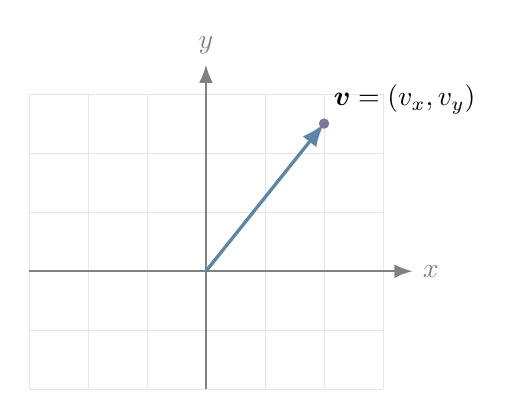
\begin{tikzpicture}[
    >=Latex,
    scale=0.75
]

% Grid
\draw[step=1cm, gray!20, very thin]
    (-3,-2) grid (3,3);

% Axes
\draw[->, thick, gray]
    (-3,0) -- (3.5,0)
    node[right] {$x$};

\draw[->, thick, gray]
    (0,-2) -- (0,3.5)
    node[above] {$y$};

% Vector
\draw[->, very thick, PastelBlue]
    (0,0) -- (2,2.5);

% Point
\fill[PastelLavender]
    (2,2.5) circle (2.5pt);

% Vector label
\node[above right] at (2,2.5)
    {$\vect{v}=(v_x,v_y)$};

\end{tikzpicture}

\end{center}

\end{column}

\end{columns}

\end{frame}

% =========================================================
% VECTOR AS A COLUMN
% =========================================================

\begin{frame}{Representing Vectors}

Vectors are commonly written as column vectors:
\[
\vect{v}
=
\begin{bmatrix}
v_1\\
v_2\\
v_3
\end{bmatrix}
\in \mathbb{R}^3.
\]

More generally,
\[
\vect{v}
=
\begin{bmatrix}
v_1\\
v_2\\
\vdots\\
v_n
\end{bmatrix}
\in \mathbb{R}^n.
\]

\begin{block}{Interpretation}
A vector in $\mathbb{R}^n$ has $n$ components and can be viewed as a point or a directed quantity in an $n$-dimensional space.
\end{block}

\end{frame}


% =========================================================
% VECTOR ADDITION
% =========================================================

\begin{frame}{Vector Addition}

Two vectors of the same dimension can be added component-wise.

\[
\vect{u}
=
\begin{bmatrix}
u_1\\
u_2
\end{bmatrix},
\qquad
\vect{v}
=
\begin{bmatrix}
v_1\\
v_2
\end{bmatrix}
\]

give

\[
\boxed{
\vect{u}+\vect{v}
=
\begin{bmatrix}
u_1+v_1\\
u_2+v_2
\end{bmatrix}
}
\]

\vspace{0.4cm}

\begin{exampleblock}{Example}
\[
\begin{bmatrix}
2\\
1
\end{bmatrix}
+
\begin{bmatrix}
3\\
4
\end{bmatrix}
=
\begin{bmatrix}
5\\
5
\end{bmatrix}
\]
\end{exampleblock}

\end{frame}


% =========================================================
% GEOMETRIC VECTOR ADDITION
% =========================================================

\begin{frame}{Geometric Interpretation of Addition}

Vector addition can be visualized using the \textbf{parallelogram rule}.

\vspace{0.2cm}

\begin{center}

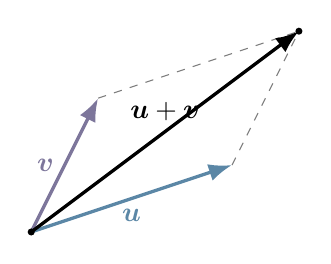
\begin{tikzpicture}[
    >=Latex,
    scale=0.85
]

\coordinate (O) at (0,0);
\coordinate (U) at (3,1);
\coordinate (V) at (1,2);
\coordinate (W) at (4,3);

\draw[->, very thick, PastelBlue]
    (O) -- (U)
    node[midway, below] {$\vect{u}$};

\draw[->, very thick, PastelLavender]
    (O) -- (V)
    node[midway, left] {$\vect{v}$};

\draw[dashed, gray]
    (U) -- (W);

\draw[dashed, gray]
    (V) -- (W);

\draw[->, very thick]
    (O) -- (W)
    node[midway, above] {$\vect{u}+\vect{v}$};

\fill (O) circle (1.5pt);
\fill (W) circle (1.5pt);

\end{tikzpicture}

\end{center}

\end{frame}


% =========================================================
% SCALAR MULTIPLICATION
% =========================================================

\begin{frame}{Scalar Multiplication}

A \textbf{scalar} is a number that can scale a vector.

For a scalar $c$,

\begin{columns}[c,totalwidth=\textwidth]

% ---------- LEFT ----------
\begin{column}{0.45\textwidth}

\begin{center}

\[
\vect{v}
=
\begin{bmatrix}
v_1\\
v_2\\
\vdots\\
v_n
\end{bmatrix}
\]

\end{center}

\end{column}

% ---------- RIGHT ----------
\begin{column}{0.45\textwidth}

\begin{center}

\[
c\vect{v}
=
\begin{bmatrix}
cv_1\\
cv_2\\
\vdots\\
cv_n
\end{bmatrix}
\]

\end{center}

\end{column}

\end{columns}

\vspace{0.4cm}

\begin{itemize}
    \item $|c|>1$   : vector is stretched
    \item $0<|c|<1$ : vector is shortened
    \item $c<0$     : direction is reversed
\end{itemize}

\end{frame}

% =========================================================
% VECTOR MAGNITUDE
% =========================================================

\begin{frame}{Magnitude of a Vector}

The magnitude or Euclidean norm measures the length of a vector.

For
\vspace{-0.5cm}

\begin{center}

\[
\vect{v}
=
\begin{bmatrix}
v_1\\
v_2
\end{bmatrix}
\qquad
\boxed{
\|\vect{v}\|
=
\sqrt{v_1^2+v_2^2}
}
\]

\end{center}

\vspace{-0.5cm}

\noindent For $\vect{v}\in\mathbb{R}^n$,

\begin{center}

\[
\boxed{
\|\vect{v}\|
=
\sqrt{
\sum_{i=1}^{n} v_i^2
}
}
\]

\end{center}

\vspace{-0.2cm}

\begin{exampleblock}{Example}

\[
\vect{v}
=
\begin{bmatrix}
3\\
4
\end{bmatrix}
\quad\Longrightarrow\quad
\|\vect{v}\|
=
\sqrt{3^2+4^2}
=
5
\]

\end{exampleblock}

\end{frame}


% =========================================================
% DISTANCE BETWEEN VECTORS
% =========================================================

\begin{frame}{Distance Between Vectors}

The distance between two vectors is the magnitude of their difference.

For $\vect{u},\vect{v}\in\mathbb{R}^n$,

\[
\boxed{
d(\vect{u},\vect{v})
=
\|\vect{u}-\vect{v}\|
}
\]

\vspace{0.5cm}

For example,

\[
\vect{u}
=
\begin{bmatrix}
3\\
4
\end{bmatrix},
\qquad
\vect{v}
=
\begin{bmatrix}
1\\
1
\end{bmatrix}
\]

give

\[
d(\vect{u},\vect{v})
=
\left\|
\begin{bmatrix}
2\\
3
\end{bmatrix}
\right\|
=
\sqrt{13}.
\]

\end{frame}


% =========================================================
% VECTORS IN COMPUTING
% =========================================================

\begin{frame}{Vectors in Computing}

Vectors provide a common representation for numerical information.

\vspace{0.3cm}

\begin{columns}[T,totalwidth=\textwidth]

\begin{column}{0.31\textwidth}

\begin{block}{Machine Learning}
Feature vectors represent measurable properties of an observation.
\end{block}

\end{column}

\begin{column}{0.31\textwidth}

\begin{block}{Computer Graphics}
Coordinates and transformations can be represented using vectors.
\end{block}

\end{column}

\begin{column}{0.31\textwidth}

\begin{block}{Data Representation}
Objects such as documents or records can be represented numerically.
\end{block}

\end{column}

\end{columns}

\vspace{0.5cm}

\begin{center}
\[
\boxed{
\text{Real-world information}
\quad\longrightarrow\quad
\text{Numerical vector}
}
\]
\end{center}

\end{frame}
% =========================================================
% 02_vector_operations.tex
% Vectors and Linear Algebra
% =========================================================

% =========================================================
% SECTION DIVIDER
% =========================================================

\section{Dot Products and Geometry}

\begin{frame}{Dot Product}

For two vectors
\[
\vect{u}
=
\begin{bmatrix}
u_1\\
u_2\\
\vdots\\
u_n
\end{bmatrix},
\qquad
\vect{v}
=
\begin{bmatrix}
v_1\\
v_2\\
\vdots\\
v_n
\end{bmatrix},
\]

their \textbf{dot product} is
\[
\boxed{
\vect{u}\cdot\vect{v}
=
\sum_{i=1}^{n}u_i v_i
}
\]

or equivalently,

\[
\boxed{
\vect{u}\cdot\vect{v}
=
\vect{u}^{T}\vect{v}
}
\]

\end{frame}


% =========================================================
% EXAMPLE
% =========================================================

\begin{frame}{Dot Product: Example}

Consider

\[
\vect{u}
=
\begin{bmatrix}
2\\
3
\end{bmatrix},
\qquad
\vect{v}
=
\begin{bmatrix}
4\\
-1
\end{bmatrix}.
\]

Then

\[
\begin{aligned}
\vect{u}\cdot\vect{v}
&=
(2)(4)+(3)(-1)\\
&=8-3\\
&=5.
\end{aligned}
\]

Therefore,

\[
\boxed{\vect{u}\cdot\vect{v}=5}
\]

The dot product of two vectors is a \textbf{scalar}, not a vector.

\end{frame}


% =========================================================
% GEOMETRIC FORM
% =========================================================

\begin{frame}{Geometric Interpretation of the Dot Product}

The dot product can also be expressed as

\[
\boxed{
\vect{u}\cdot\vect{v}
=
\|\vect{u}\|
\|\vect{v}\|
\cos\theta
}
\]

where $\theta$ is the angle between the vectors.

\vspace{0.4cm}

Therefore,

\[
\boxed{
\cos\theta
=
\frac{
\vect{u}\cdot\vect{v}
}{
\|\vect{u}\|\|\vect{v}\|
}
}
\]

\vspace{0.3cm}

The dot product therefore connects:

\[
\text{algebra}
\quad\longleftrightarrow\quad
\text{geometry}.
\]

\end{frame}


% =========================================================
% ANGLE BETWEEN VECTORS
% =========================================================

\begin{frame}{Angle Between Two Vectors}

For non-zero vectors $\vect{u}$ and $\vect{v}$,

\[
\boxed{
\theta
=
\cos^{-1}
\left(
\frac{
\vect{u}\cdot\vect{v}
}{
\|\vect{u}\|\|\vect{v}\|
}
\right)
}
\]

\vspace{0.5cm}

The sign of the dot product provides useful geometric information:

\begin{itemize}
    \item $\vect{u}\cdot\vect{v}>0$: acute angle
    \item $\vect{u}\cdot\vect{v}=0$: right angle
    \item $\vect{u}\cdot\vect{v}<0$: obtuse angle
\end{itemize}

\end{frame}


% =========================================================
% ORTHOGONALITY
% =========================================================

\begin{frame}{Orthogonal Vectors}

Two vectors are \textbf{orthogonal} if they are perpendicular.

For vectors $\vect{u}$ and $\vect{v}$,

\vspace{-0.5cm}
\[
\boxed{
\vect{u}\cdot\vect{v}=0
}
\]

implies

\vspace{-0.5cm}
\[
\boxed{
\vect{u}\perp\vect{v}
}
\]

provided both vectors are non-zero.

\begin{exampleblock}{Example}
\[
\vect{u}
=
\begin{bmatrix}
2\\
1
\end{bmatrix},
\qquad
\vect{v}
=
\begin{bmatrix}
1\\
-2
\end{bmatrix}
\]

\vspace{-0.2cm}

Since
\[
\vect{u}\cdot\vect{v}
=
2(1)+1(-2)=0,
\]
the vectors are orthogonal.

\end{exampleblock}

\end{frame}


% =========================================================
% ORTHOGONAL PROJECTION
% =========================================================

\begin{frame}{Orthogonal Projection}

The projection of $\vect{u}$ onto a non-zero vector $\vect{v}$ is

\[
\boxed{
\operatorname{proj}_{\vect{v}}(\vect{u})
=
\frac{
\vect{u}\cdot\vect{v}
}{
\vect{v}\cdot\vect{v}
}
\vect{v}
}
\]

\vspace{0.5cm}

The projection gives the component of $\vect{u}$ that lies in the direction of $\vect{v}$.

\vspace{0.3cm}

It is useful in:

\begin{itemize}
    \item geometry
    \item least-squares methods
    \item computer graphics
    \item machine learning
\end{itemize}

\end{frame}


% =========================================================
% VECTOR DECOMPOSITION
% =========================================================

\begin{frame}{Decomposing a Vector}

A vector can be separated into components parallel and perpendicular to another vector.

\[
\boxed{
\vect{u}
=
\operatorname{proj}_{\vect{v}}(\vect{u})
+
\vect{u}_{\perp}
}
\]

where

\[
\vect{u}_{\perp}
=
\vect{u}
-
\operatorname{proj}_{\vect{v}}(\vect{u}).
\]

\vspace{0.4cm}

The two components satisfy

\[
\boxed{
\vect{u}_{\perp}\cdot\vect{v}=0.
}
\]

\end{frame}


% =========================================================
% DOT PRODUCT AND DISTANCE
% =========================================================

\begin{frame}{Dot Product and Distance}

The dot product can also be used to express the squared distance between two vectors.

For $\vect{u},\vect{v}\in\mathbb{R}^n$,

\[
\|\vect{u}-\vect{v}\|^2
=
(\vect{u}-\vect{v})^T
(\vect{u}-\vect{v}).
\]

Expanding,

\[
\boxed{
\|\vect{u}-\vect{v}\|^2
=
\vect{u}^T\vect{u}
+
\vect{v}^T\vect{v}
-
2\vect{u}^T\vect{v}
}
\]

Thus the dot product is closely connected to both:

\[
\text{length}
\qquad\text{and}\qquad
\text{distance}.
\]

\end{frame}


% =========================================================
% DOT PRODUCT AS A FUNCTION
% =========================================================

\begin{frame}{Dot Product and Duality}

For a fixed vector $\vect{w}$, consider

\[
f(\vect{x})
=
\vect{w}^{T}\vect{x}.
\]

This takes a vector $\vect{x}$ and produces a scalar.

\vspace{0.4cm}

\[
\boxed{
\vect{x}
\longrightarrow
\vect{w}^{T}\vect{x}
}
\]

Such a function is a \textbf{linear functional}.

\vspace{0.4cm}

This provides a connection between:

\[
\boxed{
\text{vectors}
\quad\longleftrightarrow\quad
\text{linear functions}
}
\]

and leads naturally to the idea of \textbf{duality}.

\end{frame}


% =========================================================
% WEIGHT VECTORS
% =========================================================

\begin{frame}{Weight Vectors}

A weight vector can define a linear function
\[
f(\vect{x})
=
\vect{w}^{T}\vect{x}.
\]

For
\[
\vect{w}
=
\begin{bmatrix}
w_1\\
w_2
\end{bmatrix},
\qquad
\vect{x}
=
\begin{bmatrix}
x_1\\
x_2
\end{bmatrix},
\]

we obtain
\[
f(\vect{x})
=
w_1x_1+w_2x_2.
\]

In machine learning, weight vectors are fundamental to:

\begin{itemize}
    \item linear models
    \item linear classifiers
    \item perceptrons
\end{itemize}

\end{frame}


% =========================================================
% HYPERPLANE
% =========================================================

\begin{frame}{Hyperplanes}

A vector $\vect{w}$ can define a hyperplane through

\[
\boxed{
\vect{w}^{T}\vect{x}=c
}
\]

where $c$ is a constant.

\vspace{0.2cm}

The vector $\vect{w}$ is \textbf{normal} to the hyperplane.

\vspace{0.2cm}

In two dimensions:

\[
w_1x_1+w_2x_2=c
\]

represents a line.

In three dimensions:
\[
w_1x_1+w_2x_2+w_3x_3=c
\]

represents a plane.

\end{frame}


% =========================================================
% CLASSIFICATION INTERPRETATION
% =========================================================

\begin{frame}{Hyperplanes in Classification}

A linear classifier can use

\[
f(\vect{x})
=
\vect{w}^{T}\vect{x}+b.
\]

The decision boundary is

\[
\boxed{
\vect{w}^{T}\vect{x}+b=0
}
\]

\vspace{0.4cm}

The space can then be divided according to the sign of $f(\vect{x})$:

\[
\begin{cases}
f(\vect{x})>0 & \text{one side}\\
f(\vect{x})<0 & \text{other side}.
\end{cases}
\]

\vspace{0.4cm}

This is the geometric foundation of models such as the \textbf{perceptron}.

\end{frame}
% =========================================================
% 03_linear_combinations.tex
% Vectors and Linear Algebra
% =========================================================

% =========================================================
% SECTION DIVIDER
% =========================================================

\section{Linear Combinations and Span}

\begin{frame}{Linear Combinations}

A \textbf{linear combination} of vectors is formed by multiplying
vectors by scalars and adding the results.

For vectors $\vect{v}_1,\vect{v}_2,\ldots,\vect{v}_k$,

\[
\boxed{
\vect{w}
=
c_1\vect{v}_1
+
c_2\vect{v}_2
+\cdots+
c_k\vect{v}_k
}
\]

where $c_1,c_2,\ldots,c_k$ are scalars.

\vspace{0.4cm}

The scalars are called the \textbf{coefficients} of the linear combination.

\end{frame}


% =========================================================
% EXAMPLE
% =========================================================

\begin{frame}{Linear Combination: Example}

Let
\vspace{-0.1cm}
\[
\vect{u}
=
\begin{bmatrix}
1\\
2
\end{bmatrix},
\qquad
\vect{v}
=
\begin{bmatrix}
3\\
1
\end{bmatrix}.
\]

Consider
\vspace{-0.1cm}
\[
2\vect{u}-\vect{v}.
\]

Then
\vspace{-0.1cm}
\[
\begin{aligned}
2\vect{u}-\vect{v}
&=
2
\begin{bmatrix}
1\\
2
\end{bmatrix}
-
\begin{bmatrix}
3\\
1
\end{bmatrix}\\[4pt]
&=
\begin{bmatrix}
2\\
4
\end{bmatrix}
-
\begin{bmatrix}
3\\
1
\end{bmatrix}\\[4pt]
&=
\boxed{
\begin{bmatrix}
-1\\
3
\end{bmatrix}}
\end{aligned}
\]

\end{frame}


% =========================================================
% GEOMETRIC INTERPRETATION
% =========================================================

\begin{frame}{Linear Combinations: Geometric View}

Suppose

\[
\vect{w}=a\vect{u}+b\vect{v}.
\]

The coefficients $a$ and $b$ determine how much of each vector
contributes to $\vect{w}$.

\vspace{0.3cm}

\begin{center}

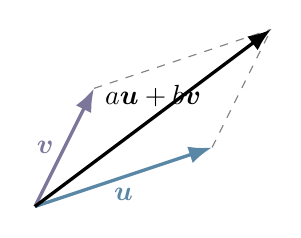
\begin{tikzpicture}[
    >=Latex,
    scale=0.75
]

\coordinate (O) at (0,0);
\coordinate (U) at (3,1);
\coordinate (V) at (1,2);
\coordinate (W) at (4,3);

\draw[->, very thick, PastelBlue]
    (O) -- (U)
    node[midway, below] {$\vect{u}$};

\draw[->, very thick, PastelLavender]
    (O) -- (V)
    node[midway, left] {$\vect{v}$};

\draw[dashed, gray] (U) -- (W);
\draw[dashed, gray] (V) -- (W);

\draw[->, very thick]
    (O) -- (W)
    node[midway, above] {$a\vect{u}+b\vect{v}$};

\end{tikzpicture}

\end{center}

\[
\boxed{\vect{w}=a\vect{u}+b\vect{v}}
\]

\end{frame}


% =========================================================
% SPAN
% =========================================================

\begin{frame}{Span of Vectors}

The \textbf{span} of a set of vectors is the set of all
possible linear combinations of those vectors.

For

\[
\vect{v}_1,\vect{v}_2,\ldots,\vect{v}_k,
\]

the span is

\[
\boxed{
\operatorname{span}
\{\vect{v}_1,\ldots,\vect{v}_k\}
=
\left\{
\sum_{i=1}^{k}c_i\vect{v}_i
\;:\;
c_i\in\mathbb{R}
\right\}
}
\]

\vspace{0.4cm}

The span describes the set of vectors that can be generated
from the given vectors.

\end{frame}


% =========================================================
% SPAN IN R2
% =========================================================

\begin{frame}{Span in $\mathbb{R}^2$}

Consider two vectors
\vspace{0.1cm}
\[
\vect{u}
=
\begin{bmatrix}
1\\
0
\end{bmatrix},
\qquad
\vect{v}
=
\begin{bmatrix}
0\\
1
\end{bmatrix}.
\]

Any vector
\vspace{0.1cm}
\[
\begin{bmatrix}
x\\
y
\end{bmatrix}
\in\mathbb{R}^2
\]

can be written as
\vspace{0.1cm}
\[
\begin{bmatrix}
x\\
y
\end{bmatrix}
=
x
\begin{bmatrix}
1\\
0
\end{bmatrix}
+
y
\begin{bmatrix}
0\\
1
\end{bmatrix}.
\]

Therefore,
\vspace{0.1cm}
\[
\boxed{
\operatorname{span}\{\vect{u},\vect{v}\}
=
\mathbb{R}^2
}
\]

\end{frame}


% =========================================================
% SPAN GEOMETRY
% =========================================================

\begin{frame}{Geometric Meaning of Span}

The span of vectors can have different dimensions.

\vspace{0.3cm}

\begin{columns}[T,totalwidth=\textwidth]

\begin{column}{0.31\textwidth}

\begin{block}{One Direction}

A non-zero vector spans a \textbf{line}.

\[
\operatorname{span}\{\vect{v}\}
\]

\end{block}

\end{column}

\begin{column}{0.31\textwidth}

\begin{block}{Two Directions}

Two independent vectors in $\mathbb{R}^2$ span a \textbf{plane}.

\[
\operatorname{span}\{\vect{u},\vect{v}\}
\]

\end{block}

\end{column}

\begin{column}{0.31\textwidth}

\begin{block}{Three Directions}

Three independent vectors in $\mathbb{R}^3$ span
three-dimensional space.

\[
\mathbb{R}^3
\]

\end{block}

\end{column}

\end{columns}

\vspace{0.5cm}

\begin{center}
The span describes the \textbf{space generated by the vectors}.
\end{center}

\end{frame}


% =========================================================
% LINEAR INDEPENDENCE
% =========================================================

\begin{frame}{Linearly Independent Vectors}

Vectors $\vect{v}_1,\ldots,\vect{v}_k$ are \textbf{linearly independent}
if the equation

\[
c_1\vect{v}_1+
c_2\vect{v}_2+
\cdots+
c_k\vect{v}_k
=
\mathbf{0}
\]

has only the trivial solution

\[
\boxed{
c_1=c_2=\cdots=c_k=0.
}
\]

\vspace{0.5cm}

In other words, none of the vectors can be written as a
linear combination of the others.

\end{frame}


% =========================================================
% LINEAR DEPENDENCE
% =========================================================

\begin{frame}{Linearly Dependent Vectors}

Vectors are \textbf{linearly dependent} if there exists a
non-trivial set of coefficients such that

\[
c_1\vect{v}_1+
c_2\vect{v}_2+
\cdots+
c_k\vect{v}_k
=
\mathbf{0},
\]

where at least one coefficient is non-zero.

\[
\boxed{
\text{Non-trivial solution}
\quad\Longrightarrow\quad
\text{Linear dependence}
}
\]

\vspace{0.4cm}

This means that at least one vector can be expressed as a
linear combination of the others.

\end{frame}


% =========================================================
% DEPENDENCE EXAMPLE
% =========================================================

\begin{frame}{Linear Dependence: Example}

Consider
\vspace{-0.1cm}
\[
\vect{u}
=
\begin{bmatrix}
1\\
2
\end{bmatrix},
\qquad
\vect{v}
=
\begin{bmatrix}
2\\
4
\end{bmatrix}.
\]

Notice that
\vspace{-0.1cm}
\[
\vect{v}=2\vect{u}.
\]

Therefore,
\vspace{-0.1cm}
\[
2\vect{u}-\vect{v}
=
\mathbf{0}.
\]

The coefficients
\vspace{-0.1cm}
\[
2\neq0,
\qquad
-1\neq0
\]

give a non-trivial solution.

Hence,

\[
\boxed{
\vect{u},\vect{v}
\text{ are linearly dependent.}
}
\]

\end{frame}


% =========================================================
% INDEPENDENCE EXAMPLE
% =========================================================

\begin{frame}{Linear Independence: Example}

Consider
\vspace{-0.1cm}
\[
\vect{u}
=
\begin{bmatrix}
1\\
0
\end{bmatrix},
\qquad
\vect{v}
=
\begin{bmatrix}
0\\
1
\end{bmatrix}.
\]

Suppose

\[
a\vect{u}+b\vect{v}
=
\mathbf{0}.
\]

Then
\vspace{-0.1cm}
\[
a
\begin{bmatrix}
1\\
0
\end{bmatrix}
+
b
\begin{bmatrix}
0\\
1
\end{bmatrix}
=
\begin{bmatrix}
0\\
0
\end{bmatrix}.
\]

Therefore,

\[
a=0,
\qquad
b=0.
\]

Hence,
\vspace{-0.1cm}
\[
\boxed{
\vect{u},\vect{v}
\text{ are linearly independent.}
}
\]

\end{frame}


% =========================================================
% LINEAR COMBINATION, SPAN, INDEPENDENCE
% =========================================================

\begin{frame}{How the Concepts Are Connected}

The ideas introduced so far are closely related:

\vspace{0.4cm}

\begin{center}

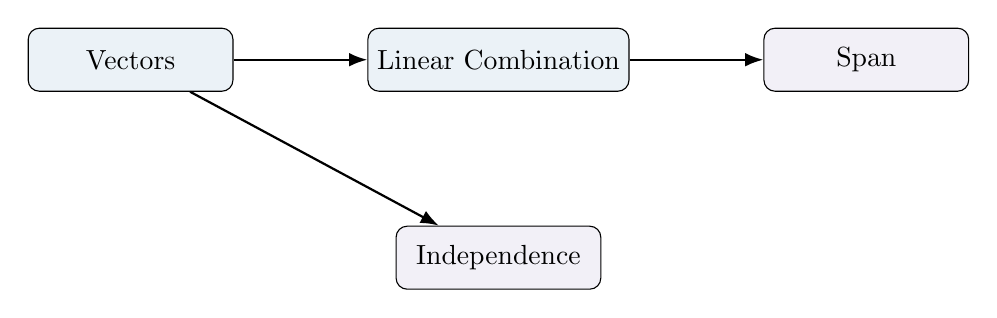
\begin{tikzpicture}[
    node distance=1.7cm,
    >=Latex
]

\node[
    draw,
    rounded corners,
    fill=LightBlue,
    minimum width=2.6cm,
    minimum height=0.8cm
] (vectors) {Vectors};

\node[
    draw,
    rounded corners,
    fill=LightBlue,
    minimum width=2.6cm,
    minimum height=0.8cm,
    right=of vectors
] (combination) {Linear Combination};

\node[
    draw,
    rounded corners,
    fill=LightLavender,
    minimum width=2.6cm,
    minimum height=0.8cm,
    right=of combination
] (span) {Span};

\node[
    draw,
    rounded corners,
    fill=LightLavender,
    minimum width=2.6cm,
    minimum height=0.8cm,
    below=of combination
] (independence) {Independence};

\draw[->, thick] (vectors) -- (combination);
\draw[->, thick] (combination) -- (span);
\draw[->, thick] (vectors) -- (independence);

\end{tikzpicture}

\end{center}

\vspace{0.4cm}

\begin{itemize}
    \item Linear combinations generate vectors.
    \item The span contains all vectors that can be generated.
    \item Linear independence describes whether the generators are redundant.
\end{itemize}

\end{frame}


% =========================================================
% LINEAR COMBINATION AND SYSTEMS
% =========================================================

\begin{frame}{Linear Combinations and Linear Systems}

Consider
\vspace{-0.1cm}
\[
A\vect{x}=\vect{b}.
\]

If
\vspace{-0.1cm}
\[
A=
\begin{bmatrix}
| & | & & |\\
\vect{a}_1 & \vect{a}_2 & \cdots & \vect{a}_n\\
| & | & & |
\end{bmatrix},
\]

then
\vspace{-0.1cm}
\[
A\vect{x}
=
x_1\vect{a}_1+
x_2\vect{a}_2+
\cdots+
x_n\vect{a}_n.
\]

Therefore,
\vspace{-0.1cm}
\[
\boxed{
A\vect{x}=\vect{b}
}
\]

asks whether $\vect{b}$ can be expressed as a linear combination
of the columns of $A$.

\vspace{0.1cm}

This connection will become important when we study
\textbf{column space and systems of linear equations}.

\end{frame}


% =========================================================
% MAXIMUM NUMBER OF INDEPENDENT VECTORS
% =========================================================

\begin{frame}{Independent Vectors and Dimension}

In $\mathbb{R}^n$, there can be at most $n$ linearly independent
vectors.

For example:

\[
\mathbb{R}^2
\quad\Rightarrow\quad
\text{at most 2 independent vectors}
\]

\[
\mathbb{R}^3
\quad\Rightarrow\quad
\text{at most 3 independent vectors}
\]

\[
\mathbb{R}^n
\quad\Rightarrow\quad
\text{at most }n\text{ independent vectors}.
\]

\vspace{0.5cm}

This observation leads naturally to the concepts of

\[
\boxed{
\text{Basis}
\qquad\text{and}\qquad
\text{Dimension}.
}
\]

\end{frame}
% =========================================================
% 04_vector_spaces_basis.tex
% Vectors and Linear Algebra
% =========================================================

% =========================================================
% SECTION DIVIDER
% =========================================================

\section{Vector Spaces, Basis and Dimension}

\begin{frame}{Basis of a Vector Space}

A set of vectors

\[
\mathcal{B}
=
\{\vect{v}_1,\vect{v}_2,\ldots,\vect{v}_n\}
\]

is a \textbf{basis} of a vector space if:

\begin{enumerate}
    \item the vectors span the space, and
    \item the vectors are linearly independent.
\end{enumerate}

Therefore,

\[
\boxed{
\text{Basis}
=
\text{Spanning set}
+
\text{Linear independence}
}
\]

\vspace{0.4cm}

A basis provides a set of fundamental directions from which
every vector in the space can be constructed.

\end{frame}


% =========================================================
% STANDARD BASIS
% =========================================================

\begin{frame}{Standard Basis}

The standard basis of $\mathbb{R}^2$ is

\[
\boxed{
\mathcal{B}
=
\left\{
\begin{bmatrix}
1\\
0
\end{bmatrix},
\begin{bmatrix}
0\\
1
\end{bmatrix}
\right\}.
}
\]

Every vector

\[
\vect{x}
=
\begin{bmatrix}
x_1\\
x_2
\end{bmatrix}
\]

can be written as

\[
\vect{x}
=
x_1
\begin{bmatrix}
1\\
0
\end{bmatrix}
+
x_2
\begin{bmatrix}
0\\
1
\end{bmatrix}.
\]

\vspace{0.3cm}

Thus, the basis vectors provide the coordinate directions of
$\mathbb{R}^2$.

\end{frame}


% =========================================================
% BASIS IN R3
% =========================================================

\begin{frame}{Standard Basis of $\mathbb{R}^3$}

The standard basis of $\mathbb{R}^3$ is

\[
\mathcal{B}
=
\left\{
\begin{bmatrix}
1\\0\\0
\end{bmatrix},
\begin{bmatrix}
0\\1\\0
\end{bmatrix},
\begin{bmatrix}
0\\0\\1
\end{bmatrix}
\right\}.
\]

Any vector

\[
\vect{x}
=
\begin{bmatrix}
x_1\\x_2\\x_3
\end{bmatrix}
\]

can be expressed as

\[
\boxed{
\vect{x}
=
x_1\vect{e}_1
+
x_2\vect{e}_2
+
x_3\vect{e}_3.
}
\]

The three basis vectors provide three independent directions.

\end{frame}


% =========================================================
% COORDINATES RELATIVE TO A BASIS
% =========================================================

\begin{frame}{Coordinates Relative to a Basis}

Let

\[
\mathcal{B}
=
\{\vect{v}_1,\vect{v}_2\}
\]

be a basis of $\mathbb{R}^2$.

A vector $\vect{x}$ can be expressed as

\[
\vect{x}
=
c_1\vect{v}_1+c_2\vect{v}_2.
\]

The coefficients form the \textbf{coordinate vector} of $\vect{x}$
relative to $\mathcal{B}$:

\[
\boxed{
[\vect{x}]_{\mathcal{B}}
=
\begin{bmatrix}
c_1\\
c_2
\end{bmatrix}.
}
\]

\vspace{0.3cm}

The same geometric vector can therefore have different coordinates
when different bases are used.

\end{frame}


% =========================================================
% DIMENSION
% =========================================================

\begin{frame}{Dimension}

The \textbf{dimension} of a vector space is the number of vectors
in any basis of that space.

For example,

\[
\boxed{
\dim(\mathbb{R}^2)=2
}
\]

and

\[
\boxed{
\dim(\mathbb{R}^3)=3.
}
\]

\vspace{0.5cm}

More generally,

\[
\boxed{
\dim(\mathbb{R}^n)=n.
}
\]

Dimension tells us how many independent directions are needed
to describe the entire space.

\end{frame}


% =========================================================
% BASIS AND DIMENSION
% =========================================================

\begin{frame}{Basis, Span and Dimension}

These concepts are closely connected.
\vspace{-0.1cm}
\[
\boxed{
\begin{array}{c}
\text{Linearly independent vectors}\\[3pt]
\downarrow\\[3pt]
\text{Basis}\\[3pt]
\downarrow\\[3pt]
\text{Spans the vector space}\\[3pt]
\downarrow\\[3pt]
\text{Number of basis vectors}\\[3pt]
\downarrow\\[3pt]
\text{Dimension}
\end{array}
}
\]

A basis is therefore a \textbf{minimal set of generators} for
a vector space.

\end{frame}


% =========================================================
% VECTOR SPACE
% =========================================================

\begin{frame}{What Is a Vector Space?}

A \textbf{vector space} is a set of objects that is closed under:

\begin{itemize}
    \item vector addition
    \item scalar multiplication
\end{itemize}

and satisfies a collection of algebraic rules.

\vspace{0.4cm}

If $\vect{u}$ and $\vect{v}$ belong to a vector space $V$, and
$c$ is a scalar, then

\[
\vect{u}+\vect{v}\in V
\]

and

\[
c\vect{u}\in V.
\]

\vspace{0.4cm}

The scalars are usually elements of $\mathbb{R}$ or $\mathbb{C}$.

\end{frame}


% =========================================================
% VECTOR SPACE AXIOMS
% =========================================================

\begin{frame}{Vector Space Properties}

For vectors $\vect{u},\vect{v},\vect{w}\in V$ and scalar $c$,
the vector-space operations satisfy properties such as:

\begin{itemize}
    \item $\vect{u}+\vect{v}=\vect{v}+\vect{u}$
    \item $(\vect{u}+\vect{v})+\vect{w}
    =\vect{u}+(\vect{v}+\vect{w})$
    \item There exists a zero vector $\mathbf{0}$
    \item Every vector has an additive inverse
    \item $c(\vect{u}+\vect{v})
    =c\vect{u}+c\vect{v}$
    \item $(c+d)\vect{u}
    =c\vect{u}+d\vect{u}$
\end{itemize}

\vspace{0.2cm}

These properties provide the algebraic structure required
for vector-space operations.

\end{frame}


% =========================================================
% EXAMPLES OF VECTOR SPACES
% =========================================================

\begin{frame}{Examples of Vector Spaces}

Vector spaces are not limited to arrows in $\mathbb{R}^n$.

Examples include:

\begin{columns}[T,totalwidth=\textwidth]

\begin{column}{0.46\textwidth}

\begin{block}{$\mathbb{R}^n$}
\[
\begin{bmatrix}
x_1\\
\vdots\\
x_n
\end{bmatrix}
\]
\end{block}

\begin{block}{Polynomials}
\[
p(x)=a_0+a_1x+\cdots+a_nx^n
\]
\end{block}

\end{column}

\begin{column}{0.46\textwidth}

\begin{block}{Matrices}
Matrices of a fixed size form a vector space under
matrix addition and scalar multiplication.
\end{block}

\begin{block}{Functions}
Suitable sets of functions can also form vector spaces.
\end{block}

\end{column}

\end{columns}

\end{frame}


% =========================================================
% SCALARS
% =========================================================

\begin{frame}{Scalars and Fields}

A \textbf{scalar} is a quantity used to multiply vectors.

Common scalar sets include

\[
\mathbb{R}
\qquad\text{and}\qquad
\mathbb{C}.
\]

\vspace{0.4cm}

A \textbf{field} provides the arithmetic structure required
for scalar operations.

\vspace{0.4cm}

For example, the real numbers $\mathbb{R}$ form a field with

\begin{itemize}
    \item addition
    \item subtraction
    \item multiplication
    \item division by non-zero numbers
\end{itemize}

\vspace{0.2cm}

Vector spaces are therefore defined relative to a chosen
field of scalars.

\end{frame}


% =========================================================
% ALGEBRAIC STRUCTURES
% =========================================================

\begin{frame}{Algebraic Structures}

The lecture material introduces increasingly structured
algebraic systems.

\vspace{0.3cm}

\begin{center}

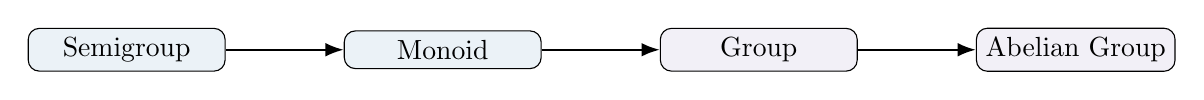
\begin{tikzpicture}[
    node distance=1.5cm,
    >=Latex
]

\node[
    draw,
    rounded corners,
    fill=LightBlue,
    minimum width=2.5cm
] (semigroup) {Semigroup};

\node[
    draw,
    rounded corners,
    fill=LightBlue,
    minimum width=2.5cm,
    right=of semigroup
] (monoid) {Monoid};

\node[
    draw,
    rounded corners,
    fill=LightLavender,
    minimum width=2.5cm,
    right=of monoid
] (group) {Group};

\node[
    draw,
    rounded corners,
    fill=LightLavender,
    minimum width=2.5cm,
    right=of group
] (abelian) {Abelian Group};

\draw[->, thick] (semigroup) -- (monoid);
\draw[->, thick] (monoid) -- (group);
\draw[->, thick] (group) -- (abelian);

\end{tikzpicture}

\end{center}

\vspace{0.4cm}

Each step adds additional algebraic properties.

\end{frame}


% =========================================================
% SEMIGROUP AND MONOID
% =========================================================

\begin{frame}{Semigroup and Monoid}

A \textbf{semigroup} is a set with an associative binary operation.

\[
(a*b)*c=a*(b*c).
\]

\vspace{0.4cm}

A \textbf{monoid} is a semigroup that additionally contains
an identity element $e$:

\[
\boxed{
e*a=a*e=a.
}
\]

\vspace{0.4cm}

These structures provide a foundation for understanding
more structured algebraic systems.

\end{frame}


% =========================================================
% GROUP
% =========================================================

\begin{frame}{Group and Abelian Group}

A \textbf{group} is a monoid in which every element has
an inverse.

For every $a$, there exists $a^{-1}$ such that

\[
aa^{-1}=a^{-1}a=e.
\]

\vspace{0.4cm}

An \textbf{Abelian group} additionally satisfies commutativity:

\[
\boxed{
a*b=b*a.
}
\]

\vspace{0.3cm}

Vector addition forms an Abelian group.

\end{frame}


% =========================================================
% VECTOR SPACE STRUCTURE
% =========================================================

\begin{frame}{From Algebraic Structure to Vector Spaces}

The vector-space structure combines two types of operations:

\vspace{0.4cm}

\begin{columns}[T,totalwidth=\textwidth]

\begin{column}{0.43\textwidth}

\begin{block}{Vector Addition}

\[
\vect{u}+\vect{v}
\]

Vectors form an Abelian group under addition.

\end{block}

\end{column}

\begin{column}{0.43\textwidth}

\begin{block}{Scalar Multiplication}

\[
c\vect{v}
\]

Scalars act on vectors while satisfying compatibility rules.

\end{block}

\end{column}

\end{columns}

\vspace{0.5cm}

Together, these operations produce the structure of a
\textbf{vector space}.

\end{frame}


% =========================================================
% VECTOR SPACES IN COMPUTING
% =========================================================

\begin{frame}{Vector Spaces in Computing}

The idea of a vector space allows many different objects
to be treated using the same mathematical framework.

\vspace{0.4cm}

\begin{itemize}
    \item Feature vectors in machine learning
    \item Coordinate vectors in computer graphics
    \item Matrix spaces in numerical computing
    \item Polynomial representations
    \item Function spaces in mathematical modelling
\end{itemize}

\begin{center}

\[
\boxed{
\text{Different objects}
\quad\longrightarrow\quad
\text{Common linear structure}
}
\]

\end{center}

\end{frame}
% =========================================================
% 05_matrices_transformations.tex
% Vectors and Linear Algebra
% =========================================================

% =========================================================
% SECTION DIVIDER
% =========================================================

\section{Matrices and Linear Transformations}

% =========================================================
% MATRICES
% =========================================================

\begin{frame}{Matrices}

A matrix is a rectangular array of numbers.

\[
A=
\begin{bmatrix}
a_{11} & a_{12}\\
a_{21} & a_{22}
\end{bmatrix}.
\]

\vspace{0.4cm}

A matrix with $m$ rows and $n$ columns has dimensions

\[
\boxed{m\times n}.
\]

\vspace{0.4cm}

Matrices can represent:

\begin{itemize}
    \item systems of linear equations
    \item transformations
    \item datasets
    \item relationships between variables
\end{itemize}

\end{frame}


% =========================================================
% MATRIX-VECTOR MULTIPLICATION
% =========================================================

\begin{frame}{Matrix--Vector Multiplication}

Let

\[
A=
\begin{bmatrix}
a_{11} & a_{12}\\
a_{21} & a_{22}
\end{bmatrix},
\qquad
\vect{x}
=
\begin{bmatrix}
x_1\\
x_2
\end{bmatrix}.
\]

Then

\[
A\vect{x}
=
\begin{bmatrix}
a_{11}x_1+a_{12}x_2\\
a_{21}x_1+a_{22}x_2
\end{bmatrix}.
\]

\vspace{0.4cm}

Equivalently,

\[
\boxed{
A\vect{x}
=
x_1
\begin{bmatrix}
a_{11}\\
a_{21}
\end{bmatrix}
+
x_2
\begin{bmatrix}
a_{12}\\
a_{22}
\end{bmatrix}
}
\]

So matrix--vector multiplication is a linear combination
of the columns of $A$.

\end{frame}


% =========================================================
% MATRIX AS A TRANSFORMATION
% =========================================================

\begin{frame}{A Matrix as a Transformation}

A matrix can define a function
\vspace{-0.1cm}
\[
T:\mathbb{R}^n\rightarrow\mathbb{R}^m
\]

through
\[
\boxed{
T(\vect{x})=A\vect{x}.
}
\]

The matrix $A$ determines how the input vector is transformed.

\[
\boxed{
\vect{x}
\quad\xrightarrow{\quad A\quad}\quad
A\vect{x}
}
\]

If

\[
A\in\mathbb{R}^{m\times n},
\]

then

\[
\vect{x}\in\mathbb{R}^n
\quad\Longrightarrow\quad
A\vect{x}\in\mathbb{R}^m.
\]

\end{frame}


% =========================================================
% LINEAR TRANSFORMATION
% =========================================================

\begin{frame}{Linear Transformations}

A transformation $T$ is linear if, for all vectors $\vect{u},\vect{v}$
and scalars $c$,

\[
\boxed{
T(\vect{u}+\vect{v})
=
T(\vect{u})+T(\vect{v})
}
\]

and

\[
\boxed{
T(c\vect{u})
=
cT(\vect{u}).
}
\]

These two properties can be combined as

\[
\boxed{
T(c_1\vect{u}+c_2\vect{v})
=
c_1T(\vect{u})+c_2T(\vect{v}).
}
\]

\end{frame}


% =========================================================
% EXAMPLE OF TRANSFORMATION
% =========================================================

\begin{frame}{Example: Scaling Transformation}

Consider
\vspace{-0.1cm}
\[
A=
\begin{bmatrix}
2&0\\
0&3
\end{bmatrix}.
\]

For
\vspace{-0.1cm}
\[
\vect{x}
=
\begin{bmatrix}
x\\
y
\end{bmatrix},
\]

we obtain

\[
A\vect{x}
=
\begin{bmatrix}
2x\\
3y
\end{bmatrix}.
\]

Therefore, the transformation

\[
T(\vect{x})=A\vect{x}
\]

scales the $x$-coordinate by $2$ and the $y$-coordinate
by $3$.

\end{frame}


% =========================================================
% IDENTITY TRANSFORMATION
% =========================================================

\begin{frame}{Identity Transformation}

The identity matrix is

\[
I=
\begin{bmatrix}
1&0\\
0&1
\end{bmatrix}.
\]

For any vector $\vect{x}$,

\[
\boxed{
I\vect{x}=\vect{x}.
}
\]

The corresponding transformation

\[
T(\vect{x})=I\vect{x}
\]

leaves every vector unchanged.
\vspace{0.1cm}

Thus, the identity transformation acts as the
\textbf{neutral transformation} under composition.

\end{frame}


% =========================================================
% ROTATION
% =========================================================

\begin{frame}{Rotation as a Linear Transformation}

A rotation through angle $\theta$ in $\mathbb{R}^2$ is represented by

\[
\boxed{
R_\theta
=
\begin{bmatrix}
\cos\theta & -\sin\theta\\
\sin\theta & \cos\theta
\end{bmatrix}.
}
\]

Therefore,

\[
T(\vect{x})
=
R_\theta\vect{x}.
\]

\vspace{0.4cm}

For $\theta=90^\circ$,

\[
R_{90^\circ}
=
\begin{bmatrix}
0&-1\\
1&0
\end{bmatrix}.
\]

\vspace{0.3cm}

The transformation rotates every vector by $90^\circ$.

\end{frame}


% =========================================================
% REFLECTION
% =========================================================

\begin{frame}{Reflection as a Linear Transformation}

Reflection about the $x$-axis can be represented by

\[
\boxed{
A=
\begin{bmatrix}
1&0\\
0&-1
\end{bmatrix}.
}
\]

For

\[
\vect{x}
=
\begin{bmatrix}
x\\
y
\end{bmatrix},
\]

we obtain

\[
A\vect{x}
=
\begin{bmatrix}
x\\
-y
\end{bmatrix}.
\]

\vspace{0.4cm}

The $x$-coordinate remains unchanged while the
$y$-coordinate changes sign.

\end{frame}


% =========================================================
% MATRIX COLUMNS AS TRANSFORMED BASIS VECTORS
% =========================================================

\begin{frame}{Columns Determine the Transformation}

Let
\vspace{-0.1cm}
\[
A=
\begin{bmatrix}
|&|\\
\vect{a}_1&\vect{a}_2\\
|&|
\end{bmatrix}.
\]

For
\vspace{-0.1cm}
\[
\vect{x}
=
\begin{bmatrix}
x_1\\
x_2
\end{bmatrix},
\]

we have
\vspace{-0.1cm}
\[
A\vect{x}
=
x_1\vect{a}_1+x_2\vect{a}_2.
\]

In particular,
\vspace{-0.1cm}
\[
A
\begin{bmatrix}
1\\
0
\end{bmatrix}
=
\vect{a}_1,
\qquad
A
\begin{bmatrix}
0\\
1
\end{bmatrix}
=
\vect{a}_2.
\]

Thus, the columns of a matrix are the images of the
standard basis vectors.

\end{frame}


% =========================================================
% COMPOSITION
% =========================================================

\begin{frame}{Composition of Transformations}

Suppose two linear transformations are represented by

\[
T(\vect{x})=A\vect{x}
\]

and

\[
S(\vect{x})=B\vect{x}.
\]

Applying $T$ first and then $S$ gives
\vspace{-0.1cm}
\[
S(T(\vect{x}))
=
B(A\vect{x}).
\]

Therefore,
\vspace{-0.1cm}
\[
\boxed{
S\circ T
\quad\longleftrightarrow\quad
BA.
}
\]
\vspace{-0.1cm}

Matrix multiplication therefore provides a compact way to
represent the \textbf{composition of linear transformations}.

\end{frame}


% =========================================================
% ORDER MATTERS
% =========================================================

\begin{frame}{Order of Composition Matters}

In general,

\[
\boxed{
AB\neq BA.
}
\]

Therefore,

\[
B(A\vect{x})
\neq
A(B\vect{x})
\]

in general.

\vspace{0.5cm}

This means that applying transformation $A$ followed by $B$
is generally different from applying $B$ followed by $A$.

\vspace{0.4cm}

\begin{block}{Key Idea}
Matrix multiplication is generally \textbf{not commutative}.
\end{block}

\end{frame}


% =========================================================
% COMPOSITION EXAMPLE
% =========================================================

\begin{frame}{Composition: Example}

Consider

\[
A=
\begin{bmatrix}
2&0\\
0&1
\end{bmatrix},
\qquad
B=
\begin{bmatrix}
1&0\\
0&3
\end{bmatrix}.
\]

Then

\[
BA
=
\begin{bmatrix}
2&0\\
0&3
\end{bmatrix}.
\]

For this particular pair,

\[
AB=BA.
\]

But this is not generally true.

For transformations such as rotations, reflections,
and shears, the order can produce different results.

\end{frame}


% =========================================================
% THREE-DIMENSIONAL TRANSFORMATIONS
% =========================================================

\begin{frame}{Three-Dimensional Linear Transformations}

A linear transformation in three dimensions has the form

\[
\boxed{
T:\mathbb{R}^3\rightarrow\mathbb{R}^3
}
\]

with
\vspace{-0.1cm}
\[
T(\vect{x})=A\vect{x},
\]

where
\vspace{-0.1cm}
\[
A=
\begin{bmatrix}
a_{11}&a_{12}&a_{13}\\
a_{21}&a_{22}&a_{23}\\
a_{31}&a_{32}&a_{33}
\end{bmatrix}.
\]

The matrix can represent transformations such as:

\begin{itemize}
    \item scaling
    \item rotation
    \item reflection
    \item shear
\end{itemize}

\end{frame}


% =========================================================
% 3D SCALING
% =========================================================

\begin{frame}{3D Scaling}

A three-dimensional scaling transformation can be written as

\[
A=
\begin{bmatrix}
s_x&0&0\\
0&s_y&0\\
0&0&s_z
\end{bmatrix}.
\]

Then

\[
\begin{bmatrix}
x'\\
y'\\
z'
\end{bmatrix}
=
A
\begin{bmatrix}
x\\
y\\
z
\end{bmatrix}
\]

gives
\vspace{-0.1cm}
\[
\boxed{
x'=s_xx,\qquad
y'=s_yy,\qquad
z'=s_zz.
}
\]

Different scaling factors can independently stretch or
compress the three coordinate directions.

\end{frame}


% =========================================================
% 3D ROTATION
% =========================================================

\begin{frame}{Rotation About the $z$-Axis}

A rotation through $\theta$ about the $z$-axis is represented by

\[
\boxed{
R_z(\theta)
=
\begin{bmatrix}
\cos\theta&-\sin\theta&0\\
\sin\theta&\cos\theta&0\\
0&0&1
\end{bmatrix}.
}
\]

\vspace{0.4cm}

The $x$ and $y$ coordinates rotate in their plane while
the $z$ coordinate remains unchanged.

\vspace{0.4cm}

This type of transformation is fundamental in

\[
\text{3D graphics}
\qquad\text{and}\qquad
\text{computer vision}.
\]

\end{frame}


% =========================================================
% TRANSFORMATION PIPELINE
% =========================================================

\begin{frame}{Transformation Pipeline}

Multiple transformations can be combined into a single matrix.

\[
\vect{x}
\xrightarrow{\ A\ }
A\vect{x}
\xrightarrow{\ B\ }
BA\vect{x}
\xrightarrow{\ C\ }
CBA\vect{x}.
\]

Therefore,

\[
\boxed{
T(\vect{x})=CBA\vect{x}.
}
\]

\vspace{0.5cm}

This idea is central to transformation pipelines in:

\begin{itemize}
    \item computer graphics
    \item robotics
    \item computer vision
    \item geometric modelling
\end{itemize}

\end{frame}


% =========================================================
% HOMOGENEOUS COORDINATES PREVIEW
% =========================================================

\begin{frame}{Beyond Linear Transformations}

Pure linear transformations preserve the origin:

\[
\boxed{
T(\mathbf{0})=\mathbf{0}.
}
\]

Translations do not satisfy this property.

\vspace{0.4cm}

In computer graphics, translations are commonly incorporated
using \textbf{homogeneous coordinates}.

For example,

\[
\begin{bmatrix}
x'\\
y'\\
1
\end{bmatrix}
=
\begin{bmatrix}
1&0&t_x\\
0&1&t_y\\
0&0&1
\end{bmatrix}
\begin{bmatrix}
x\\
y\\
1
\end{bmatrix}.
\]

This allows translation and linear transformations to be
combined into matrix operations.

\end{frame}
% =========================================================
% 06_systems_of_linear_equations.tex
% Vectors and Linear Algebra
% =========================================================

% =========================================================
% SECTION DIVIDER
% =========================================================

\section{Systems of Linear Equations}

% =========================================================
% SYSTEM OF LINEAR EQUATIONS
% =========================================================

\begin{frame}{System of Linear Equations}

A \textbf{linear equation} in variables
$x_1,x_2,\ldots,x_n$ has the form

\[
a_1x_1+a_2x_2+\cdots+a_nx_n=b.
\]

A \textbf{system of linear equations} consists of
multiple linear equations considered simultaneously.

\vspace{0.4cm}

For example,

\[
\begin{cases}
2x+y=5,\\
x-y=1.
\end{cases}
\]

\vspace{0.3cm}

The objective is to find values of the variables that
satisfy \textbf{all equations simultaneously}.

\end{frame}


% =========================================================
% SOLUTION OF A SYSTEM
% =========================================================

\begin{frame}{Solution of a System}

For the system
\vspace{-0.1cm}
\[
\begin{cases}
2x+y=5,\\
x-y=1,
\end{cases}
\]

adding the two equations gives
\vspace{-0.1cm}
\[
3x=6.
\]

Therefore,
\vspace{-0.1cm}
\[
x=2.
\]

Substituting into
\vspace{-0.1cm}
\[
x-y=1
\]

gives
\vspace{-0.1cm}
\[
y=1.
\]

Hence,
\vspace{-0.1cm}
\[
\boxed{
(x,y)=(2,1)
}
\]
\vspace{-0.1cm}
is the solution.

\end{frame}


% =========================================================
% GEOMETRIC INTERPRETATION
% =========================================================

\begin{frame}{Geometric Interpretation}

In two variables, each linear equation represents a line.

For example,

\[
2x+y=5
\]

and

\[
x-y=1
\]

represent two lines in the plane.

\vspace{0.4cm}

Their solution is the point where the two lines intersect.

\[
\boxed{
\text{Solution of system}
=
\text{Common intersection}
}
\]

This geometric interpretation becomes more general when
we move to higher dimensions.

\end{frame}


% =========================================================
% CONSISTENCY
% =========================================================

\begin{frame}{Consistency of a System}

A system of linear equations is \textbf{consistent} if it has
at least one solution.

It is \textbf{inconsistent} if it has no solution.

\vspace{0.5cm}

A consistent system may have:

\[
\boxed{
\text{Exactly one solution}
}
\]

or

\[
\boxed{
\text{Infinitely many solutions}.
}
\]

\vspace{0.4cm}

Therefore, the three possibilities are:

\[
\boxed{
\text{Unique solution}
\qquad
\text{Infinitely many solutions}
\qquad
\text{No solution}
}
\]

\end{frame}


% =========================================================
% CONSISTENCY GEOMETRICALLY
% =========================================================

\begin{frame}{Consistency: Geometric View}

For two equations in two variables:

\vspace{0.3cm}

\begin{columns}[T,totalwidth=\textwidth]

\begin{column}{0.30\textwidth}

\begin{block}{One Solution}
Two distinct lines intersect at one point.
\end{block}

\end{column}

\begin{column}{0.30\textwidth}

\begin{block}{No Solution}
Parallel distinct lines never intersect.
\end{block}

\end{column}

\begin{column}{0.30\textwidth}

\begin{block}{Infinite Solutions}
Coincident lines represent the same equation.
\end{block}

\end{column}

\end{columns}

\vspace{0.5cm}

Thus, consistency is closely related to the geometry of the
equations.

\end{frame}


% =========================================================
% MATRIX FORM
% =========================================================

\begin{frame}{Matrix Form of a Linear System}

Consider

\[
\begin{cases}
a_{11}x_1+a_{12}x_2=b_1,\\
a_{21}x_1+a_{22}x_2=b_2.
\end{cases}
\]

Define

\[
A=
\begin{bmatrix}
a_{11}&a_{12}\\
a_{21}&a_{22}
\end{bmatrix},
\qquad
\vect{x}
=
\begin{bmatrix}
x_1\\
x_2
\end{bmatrix},
\qquad
\vect{b}
=
\begin{bmatrix}
b_1\\
b_2
\end{bmatrix}.
\]

Then the system becomes

\[
\boxed{
A\vect{x}=\vect{b}.
}
\]

\end{frame}


% =========================================================
% Ax = b
% =========================================================

\begin{frame}{The Equation $A\vect{x}=\vect{b}$}

The matrix equation

\[
\boxed{
A\vect{x}=\vect{b}
}
\]

can be interpreted as a transformation.

\[
\vect{x}
\xrightarrow{\quad A\quad}
A\vect{x}
=
\vect{b}.
\]

\vspace{0.5cm}

The problem is therefore:

\[
\boxed{
\text{Find the input }\vect{x}
\text{ that produces the output }\vect{b}.
}
\]

\vspace{0.4cm}

This connects systems of equations directly with
\textbf{linear transformations}.

\end{frame}


% =========================================================
% COLUMN INTERPRETATION
% =========================================================

\begin{frame}{$A\vect{x}=\vect{b}$ as a Linear Combination}

Let
\vspace{-1.9cm}
\begin{columns}[c,totalwidth=\textwidth]

% ---------- LEFT ----------
\begin{column}{0.45\textwidth}

\begin{center}

\[
A=
\begin{bmatrix}
|&|& &|\\
\vect{a}_1&\vect{a}_2&\cdots&\vect{a}_n\\
|&|& &|
\end{bmatrix}
\],

\end{center}

\end{column}

% ---------- RIGHT ----------
\begin{column}{0.45\textwidth}

\begin{center}

\[
\vect{x}
=
\begin{bmatrix}
x_1\\
x_2\\
\vdots\\
x_n
\end{bmatrix}
\]

\end{center}

\end{column}

\end{columns}

\vspace{0.1cm}

Then
\vspace{-0.1cm}
\[
A\vect{x}
=
x_1\vect{a}_1+
x_2\vect{a}_2+
\cdots+
x_n\vect{a}_n.
\]

Therefore,

\[
A\vect{x}=\vect{b}
\]

asks whether $\vect{b}$ can be expressed as a linear
combination of the columns of $A$.

\vspace{-0.1cm}

\begin{center}

\[
\boxed{
\vect{b}\in\operatorname{Col}(A)
}
\]

\end{center}

This is precisely the condition for consistency.

\end{frame}


% =========================================================
% AUGMENTED MATRIX
% =========================================================

\begin{frame}{Augmented Matrix}

A system can be represented using an \textbf{augmented matrix}.

For

\[
\begin{cases}
2x+y=5,\\
x-y=1,
\end{cases}
\]

the augmented matrix is

\[
\boxed{
\left[
\begin{array}{cc|c}
2&1&5\\
1&-1&1
\end{array}
\right].
}
\]

\vspace{0.4cm}

The vertical line separates:

\[
\text{coefficient matrix}
\qquad\text{from}\qquad
\text{right-hand side}.
\]

\end{frame}


% =========================================================
% ELEMENTARY ROW OPERATIONS
% =========================================================

\begin{frame}{Elementary Row Operations}

Gaussian elimination uses three elementary row operations.

\vspace{0.4cm}

\begin{enumerate}
    \item Interchange two rows.
    \item Multiply a row by a non-zero scalar.
    \item Add a multiple of one row to another row.
\end{enumerate}

\vspace{0.5cm}

These operations transform the system into an equivalent
system with the same solution set.

\[
\boxed{
\text{Equivalent system}
\quad\Longrightarrow\quad
\text{Same solutions}
}
\]

\end{frame}


% =========================================================
% GAUSSIAN ELIMINATION
% =========================================================

\begin{frame}{Gaussian Elimination}

Gaussian elimination transforms an augmented matrix into
\textbf{row echelon form}.

Consider
\vspace{-0.1cm}
\[
\left[
\begin{array}{cc|c}
2&1&5\\
1&-1&1
\end{array}
\right].
\]

Swap the rows:
\vspace{-0.1cm}
\[
\left[
\begin{array}{cc|c}
1&-1&1\\
2&1&5
\end{array}
\right].
\]

Then perform

\[
R_2\leftarrow R_2-2R_1.
\]

This gives

\[
\left[
\begin{array}{cc|c}
1&-1&1\\
0&3&3
\end{array}
\right].
\]

\end{frame}


% =========================================================
% BACK SUBSTITUTION
% =========================================================

\begin{frame}{Gaussian Elimination: Back Substitution}

From
\vspace{-0.1cm}
\[
\left[
\begin{array}{cc|c}
1&-1&1\\
0&3&3
\end{array}
\right]
\]

we obtain
\vspace{-0.1cm}
\[
3y=3
\]

and therefore
\vspace{-0.1cm}
\[
y=1.
\]

Substituting into the first equation,
\vspace{-0.2cm}
\[
x-y=1
\]

gives
\vspace{-0.2cm}
\[
x=2.
\]

Hence,
\vspace{-0.2cm}
\[
\boxed{
\vect{x}
=
\begin{bmatrix}
2\\
1
\end{bmatrix}.
}
\]

\end{frame}


% =========================================================
% ROW ECHELON FORM
% =========================================================

\begin{frame}{Row Echelon Form}

A matrix is in \textbf{row echelon form} when:

\begin{itemize}
    \item all non-zero rows occur above zero rows,
    \item each leading entry is to the right of the leading
    entry in the row above it,
    \item entries below each leading entry are zero.
\end{itemize}

For example,

\[
\begin{bmatrix}
1&2&-1\\
0&1&3\\
0&0&1
\end{bmatrix}
\]

is in row echelon form.

\vspace{0.4cm}

Gaussian elimination systematically produces this structure.

\end{frame}


% =========================================================
% REDUCED ROW ECHELON FORM
% =========================================================

\begin{frame}{Reduced Row Echelon Form}

A matrix is in \textbf{reduced row echelon form} when, in addition
to row echelon conditions:

\begin{itemize}
    \item every leading entry is $1$,
    \item each leading $1$ is the only non-zero entry in its column.
\end{itemize}

For example,

\[
\boxed{
\begin{bmatrix}
1&0&2\\
0&1&-3\\
0&0&0
\end{bmatrix}
}
\]

is in reduced row echelon form.

\vspace{0.3cm}

RREF makes the solution structure of a system easier to identify.

\end{frame}


% =========================================================
% UNIQUE SOLUTION
% =========================================================

\begin{frame}{Identifying a Unique Solution}

Consider

\[
\left[
\begin{array}{ccc|c}
1&0&2&4\\
0&1&-1&3\\
0&0&1&2
\end{array}
\right].
\]

Every variable has a pivot.

\vspace{0.4cm}

Therefore, the system has

\[
\boxed{
\text{exactly one solution}.
}
\]

In general, a unique solution occurs when every variable
is determined by the equations.

\end{frame}


% =========================================================
% NO SOLUTION
% =========================================================

\begin{frame}{Detecting No Solution}

Suppose elimination produces
\vspace{-0.1cm}
\[
\left[
\begin{array}{ccc|c}
1&2&0&3\\
0&0&0&5
\end{array}
\right].
\]

The second row represents
\vspace{-0.1cm}
\[
0=5.
\]

This is impossible.

Therefore,
\vspace{-0.1cm}
\[
\boxed{
\text{The system is inconsistent.}
}
\]

A row of the form

\[
\left[
\begin{array}{ccc|c}
0&0&0&c
\end{array}
\right],
\qquad c\neq0,
\]

signals that the system has \textbf{no solution}.

\end{frame}


% =========================================================
% INFINITELY MANY SOLUTIONS
% =========================================================

\begin{frame}{Infinitely Many Solutions}

Consider a system whose reduced form contains
\vspace{-0.1cm}
\[
\left[
\begin{array}{ccc|c}
1&0&2&4\\
0&1&-1&3\\
0&0&0&0
\end{array}
\right].
\]

The third row gives no new constraint. One variable can therefore be chosen freely.

Let
\vspace{-0.2cm}
\[
z=t.
\]

Then
\vspace{-0.1cm}
\[
x=4-2t,
\qquad
y=3+t.
\]

Hence,
\vspace{-0.1cm}
\[
\boxed{
\begin{bmatrix}
x\\y\\z
\end{bmatrix}
=
\begin{bmatrix}
4\\3\\0
\end{bmatrix}
+
t
\begin{bmatrix}
-2\\1\\1
\end{bmatrix}.
}
\]
\vspace{-0.1cm}
There are infinitely many solutions.

\end{frame}


% =========================================================
% INVERSE MATRIX
% =========================================================

\begin{frame}{Solving $A\vect{x}=\vect{b}$ Using an Inverse}
\vspace{-0.1cm}
Suppose $A$ is a square matrix with an inverse.

Starting with

\[
A\vect{x}=\vect{b},
\]

multiply both sides by $A^{-1}$:

\[
A^{-1}A\vect{x}
=
A^{-1}\vect{b}.
\]

Since
\vspace{-0.1cm}
\[
A^{-1}A=I,
\]

we obtain
\vspace{-0.1cm}
\[
\boxed{
\vect{x}=A^{-1}\vect{b}.
}
\]

This gives a direct formula for the solution.

\end{frame}


% =========================================================
% CONDITIONS FOR INVERSE SOLUTION
% =========================================================

\begin{frame}{When Does $A^{-1}\vect{b}$ Exist?}

The expression

\[
\vect{x}=A^{-1}\vect{b}
\]

requires $A$ to be:

\begin{itemize}
    \item square,
    \item invertible.
\end{itemize}

For a square matrix,

\[
A^{-1}\text{ exists}
\quad\Longleftrightarrow\quad
\det(A)\neq0.
\]


When these conditions hold, the system

\[
A\vect{x}=\vect{b}
\]

has a unique solution for every $\vect{b}$.

\end{frame}


% =========================================================
% GAUSSIAN ELIMINATION VS INVERSE
% =========================================================

\begin{frame}{Two Ways to Solve a Linear System}

For a system

\[
A\vect{x}=\vect{b},
\]

two approaches are:

\vspace{0.3cm}

\begin{columns}[T,totalwidth=\textwidth]

\begin{column}{0.44\textwidth}

\begin{block}{Gaussian Elimination}

Transform the augmented matrix and solve the resulting system.

\[
[A\mid\vect{b}]
\]

\end{block}

\end{column}

\begin{column}{0.44\textwidth}

\begin{block}{Inverse Method}

If $A$ is invertible,

\[
\vect{x}=A^{-1}\vect{b}.
\]

\end{block}

\end{column}

\end{columns}

\vspace{0.5cm}

For computational problems involving many right-hand sides,
factorization-based methods are generally more useful than
explicitly computing $A^{-1}$.

\end{frame}


% =========================================================
% HOMOGENEOUS SYSTEM
% =========================================================

\begin{frame}{Homogeneous Linear Systems}

A homogeneous system has the form

\[
\boxed{
A\vect{x}=\mathbf{0}.
}
\]

It always has at least the trivial solution

\[
\boxed{
\vect{x}=\mathbf{0}.
}
\]

\vspace{0.4cm}

Depending on $A$, there may also be non-zero solutions.

\vspace{0.4cm}

\[
\boxed{
\text{Trivial solution}
\qquad\text{vs.}\qquad
\text{Non-trivial solutions}
}
\]

This will become important when studying the
\textbf{null space} and linear dependence.

\end{frame}
% =========================================================
% 07_determinants_inverses_cramers.tex
% Vectors and Linear Algebra
% =========================================================

% =========================================================
% SECTION DIVIDER
% =========================================================

\section{Determinants and Inverse Matrices}

% =========================================================
% DETERMINANT
% =========================================================

\begin{frame}{The Determinant}

The \textbf{determinant} is a scalar associated with a
square matrix.

For a $2\times2$ matrix

\[
A=
\begin{bmatrix}
a&b\\
c&d
\end{bmatrix},
\]

the determinant is

\[
\boxed{
\det(A)=ad-bc.
}
\]

\vspace{0.4cm}

The determinant provides information about the transformation
represented by the matrix.

\vspace{0.3cm}

It also plays a central role in determining whether a matrix
is invertible.

\end{frame}


% =========================================================
% 2x2 EXAMPLE
% =========================================================

\begin{frame}{Example: Determinant of a $2\times2$ Matrix}

Consider
\vspace{-0.1cm}
\[
A=
\begin{bmatrix}
3&2\\
1&4
\end{bmatrix}.
\]

Then

\[
\det(A)
=
(3)(4)-(2)(1).
\]

Therefore,

\[
\boxed{
\det(A)=10.
}
\]

Since

\[
\det(A)\neq0,
\]

the matrix is invertible.

\end{frame}


% =========================================================
% GEOMETRIC MEANING
% =========================================================

\begin{frame}{Geometric Meaning of the Determinant}

For a $2\times2$ matrix, the absolute value
\vspace{-0.1cm}
\[
|\det(A)|
\]

represents the factor by which the transformation changes
\textbf{area}.

If
\vspace{-0.1cm}
\[
|\det(A)|>1,
\]

areas are enlarged.

If
\vspace{-0.1cm}
\[
0<|\det(A)|<1,
\]

areas are reduced.

If
\vspace{-0.1cm}
\[
\boxed{\det(A)=0},
\]

the transformation collapses the plane into a lower-dimensional
space.

\end{frame}


% =========================================================
% 3D DETERMINANT
% =========================================================

\begin{frame}{Determinant in Three Dimensions}

For a $3\times3$ matrix, the absolute value of the determinant
represents the volume-scaling factor.

\vspace{0.4cm}

\[
\boxed{
|\det(A)|
=
\text{volume scaling factor}
}
\]

For example,

\[
\det(A)=2
\]

means that the transformation doubles volumes.

\vspace{0.4cm}

A negative determinant indicates that the transformation also
reverses orientation.

\end{frame}


% =========================================================
% PROPERTIES
% =========================================================

\begin{frame}{Properties of the Determinant}

For square matrices $A$ and $B$:

\[
\boxed{
\det(AB)=\det(A)\det(B)
}
\]

and

\[
\boxed{
\det(A^T)=\det(A).
}
\]

For the identity matrix,

\[
\boxed{
\det(I)=1.
}
\]

For a scalar $c$ and an $n\times n$ matrix,

\[
\boxed{
\det(cA)=c^n\det(A).
}
\]

\end{frame}


% =========================================================
% SINGULAR MATRIX
% =========================================================

\begin{frame}{Singular and Non-Singular Matrices}

A square matrix $A$ is called \textbf{singular} if

\[
\boxed{
\det(A)=0.
}
\]

A square matrix is \textbf{non-singular} if

\[
\boxed{
\det(A)\neq0.
}
\]

\vspace{0.4cm}

Geometrically, a singular transformation collapses
space into a lower-dimensional set.

\vspace{0.4cm}

For example, a plane may be collapsed into a line.

\end{frame}


% =========================================================
% INVERTIBILITY
% =========================================================

\begin{frame}{Determinant and Invertibility}

For a square matrix $A$,

\[
\boxed{
A^{-1}\text{ exists}
\iff
\det(A)\neq0.
}
\]

Equivalently,

\[
\boxed{
\det(A)=0
\iff
A\text{ is singular}.
}
\]

Therefore, the determinant provides a quick test for
whether a square matrix has an inverse.

\vspace{0.4cm}

This connects three ideas:

\[
\boxed{
\text{Determinant}
\quad\longleftrightarrow\quad
\text{Invertibility}
\quad\longleftrightarrow\quad
\text{Unique solution}
}
\]

\end{frame}


% =========================================================
% INVERSE MATRIX
% =========================================================

\begin{frame}{Inverse Matrix}

For a square matrix $A$, its inverse $A^{-1}$ satisfies

\[
\boxed{
AA^{-1}=A^{-1}A=I.
}
\]

Therefore,
\vspace{-0.1cm}
\[
A^{-1}
\]

undoes the transformation performed by $A$.

\vspace{0.5cm}

If
\vspace{-0.1cm}
\[
\vect{y}=A\vect{x},
\]

then

\[
\boxed{
\vect{x}=A^{-1}\vect{y}.
}
\]

Thus, the inverse transformation recovers the original vector.

\end{frame}


% =========================================================
% 2x2 INVERSE
% =========================================================

\begin{frame}{Inverse of a $2\times2$ Matrix}

For
\vspace{-0.1cm}
\[
A=
\begin{bmatrix}
a&b\\
c&d
\end{bmatrix},
\]

if
\vspace{-0.1cm}
\[
ad-bc\neq0,
\]

then
\vspace{-0.1cm}
\[
\boxed{
A^{-1}
=
\frac{1}{ad-bc}
\begin{bmatrix}
d&-b\\
-c&a
\end{bmatrix}.
}
\]

The denominator is precisely
\vspace{-0.1cm}
\[
\det(A).
\]

Therefore,
\vspace{-0.1cm}
\[
\det(A)\neq0
\]

is required for the inverse to exist.

\end{frame}


% =========================================================
% INVERSE EXAMPLE
% =========================================================

\begin{frame}{Example: Computing an Inverse}

Consider
\vspace{-0.1cm}
\[
A=
\begin{bmatrix}
2&1\\
1&1
\end{bmatrix}.
\]

First,

\[
\det(A)
=
(2)(1)-(1)(1)
=
1.
\]

Therefore,

\[
A^{-1}
=
\begin{bmatrix}
1&-1\\
-1&2
\end{bmatrix}.
\]

Indeed,

\[
AA^{-1}
=
\begin{bmatrix}
1&0\\
0&1
\end{bmatrix}
=
I.
\]

\end{frame}


% =========================================================
% INVERSE AND LINEAR SYSTEM
% =========================================================

\begin{frame}{Inverse Matrix and Linear Systems}

Consider

\[
A\vect{x}=\vect{b}.
\]

If $A$ is invertible,

\[
A^{-1}A\vect{x}
=
A^{-1}\vect{b}.
\]

Therefore,

\[
\boxed{
\vect{x}=A^{-1}\vect{b}.
}
\]

\vspace{0.4cm}

Hence, an invertible coefficient matrix guarantees a
unique solution for every right-hand side $\vect{b}$.

\end{frame}


% =========================================================
% COFACTORS
% =========================================================

\begin{frame}{Cofactors}

For larger matrices, determinants can be computed using
\textbf{cofactors}.

For an element $a_{ij}$,

\[
\boxed{
C_{ij}=(-1)^{i+j}M_{ij},
}
\]

where $M_{ij}$ is the determinant obtained after deleting
row $i$ and column $j$.

\vspace{0.4cm}

For a $3\times3$ matrix,

\[
\det(A)
=
a_{11}C_{11}
+
a_{12}C_{12}
+
a_{13}C_{13}.
\]

\vspace{0.3cm}

This is called \textbf{cofactor expansion}.

\end{frame}


% =========================================================
% ADJUGATE
% =========================================================

\begin{frame}{Adjugate and the Inverse}

The matrix of cofactors is called the \textbf{cofactor matrix}.

Its transpose is the \textbf{adjugate}:

\[
\operatorname{adj}(A)
=
C^T.
\]

For an invertible matrix,

\[
\boxed{
A^{-1}
=
\frac{1}{\det(A)}
\operatorname{adj}(A).
}
\]

\vspace{0.4cm}

This provides a general formula for the inverse of a
square matrix.

\vspace{0.3cm}

For large matrices, however, direct inverse computation is
usually not the preferred computational approach.

\end{frame}


% =========================================================
% CRAMER'S RULE
% =========================================================

\begin{frame}{Cramer's Rule}

Consider the system

\[
A\vect{x}=\vect{b},
\]

where $A$ is an invertible $n\times n$ matrix.

Cramer's rule gives each component of the solution as

\[
\boxed{
x_i
=
\frac{\det(A_i)}{\det(A)},
}
\]

where $A_i$ is obtained by replacing the $i$-th column of $A$
with $\vect{b}$.

\vspace{0.4cm}

The rule requires

\[
\boxed{
\det(A)\neq0.
}
\]

\end{frame}


% =========================================================
% CRAMER 2x2
% =========================================================

\begin{frame}{Cramer's Rule for a $2\times2$ System}

Consider
\vspace{-0.1cm}
\[
\begin{cases}
a_1x+b_1y=c_1,\\
a_2x+b_2y=c_2.
\end{cases}
\]
\vspace{-0.1cm}
The coefficient determinant is
\vspace{-0.1cm}
\[
D=
\begin{vmatrix}
a_1&b_1\\
a_2&b_2
\end{vmatrix}.
\]
\vspace{-0.1cm}
For $x$,
\vspace{-0.1cm}
\[
D_x=
\begin{vmatrix}
c_1&b_1\\
c_2&b_2
\end{vmatrix}.
\]
\vspace{-0.1cm}
For $y$,
\vspace{-0.1cm}
\[
D_y=
\begin{vmatrix}
a_1&c_1\\
a_2&c_2
\end{vmatrix}.
\]
\vspace{-0.1cm}
Therefore,
\vspace{-0.1cm}
\[
\boxed{
x=\frac{D_x}{D},
\qquad
y=\frac{D_y}{D}.
}
\]

\end{frame}


% =========================================================
% CRAMER EXAMPLE
% =========================================================

\begin{frame}{Example: Cramer's Rule}

Consider
\vspace{-0.1cm}
\[
\begin{cases}
2x+y=5,\\
x-y=1.
\end{cases}
\]

The coefficient determinant is
\vspace{-0.1cm}
\[
D=
\begin{vmatrix}
2&1\\
1&-1
\end{vmatrix}
=-3.
\]

For $x$,
\vspace{-0.1cm}
\[
D_x=
\begin{vmatrix}
5&1\\
1&-1
\end{vmatrix}
=-6.
\]

For $y$,
\vspace{-0.1cm}
\[
D_y=
\begin{vmatrix}
2&5\\
1&1
\end{vmatrix}
=-3.
\]
\vspace{-0.1cm}
Hence,
\vspace{-0.1cm}
\[
\boxed{
x=2,\qquad y=1.
}
\]

\end{frame}


% =========================================================
% CRAMER'S RULE VS GAUSSIAN ELIMINATION
% =========================================================

\begin{frame}{Cramer's Rule and Gaussian Elimination}

Both methods can solve

\[
A\vect{x}=\vect{b}.
\]

\vspace{0.4cm}

\begin{columns}[T,totalwidth=\textwidth]

\begin{column}{0.43\textwidth}

\begin{block}{Cramer's Rule}

Uses determinants:

\[
x_i=
\frac{\det(A_i)}{\det(A)}.
\]

Useful for theoretical derivations and small systems.

\end{block}

\end{column}

\begin{column}{0.43\textwidth}

\begin{block}{Gaussian Elimination}

Uses elementary row operations.

Efficient and widely used for numerical computation.

\end{block}

\end{column}

\end{columns}

\vspace{0.4cm}

For large systems, repeatedly computing determinants is
computationally expensive.

\end{frame}


% =========================================================
% KEY CONNECTION
% =========================================================

\begin{frame}{The Linear Algebra Connection}
\vspace{-0.1cm}
For a square system
\vspace{-0.2cm}
\[
A\vect{x}=\vect{b},
\]
\vspace{-0.2cm}
the following ideas are connected:
\vspace{-0.09cm}
\[
\boxed{
\begin{array}{c}
\det(A)\neq0\\
\Downarrow\\
A\text{ is invertible}\\
\Downarrow\\
A^{-1}\text{ exists}\\
\Downarrow\\
A\vect{x}=\vect{b}\text{ has a unique solution}\\
\Downarrow\\
\vect{x}=A^{-1}\vect{b}
\end{array}
}
\]
\vspace{-0.1cm}

This connection will be extended further through
\textbf{column space, null space, rank, and linear independence}.

\end{frame}
% =========================================================
% 08_determinants_inverse.tex
% Vectors and Linear Algebra
% =========================================================

% =========================================================
% SECTION DIVIDER
% =========================================================

\section{Determinants and Inverse Matrices}

% =========================================================
% DETERMINANT
% =========================================================

\begin{frame}{The Determinant}

The \textbf{determinant} is a scalar associated with a
square matrix.

For a $2\times2$ matrix,

\[
A=
\begin{bmatrix}
a&b\\
c&d
\end{bmatrix},
\]

the determinant is

\[
\boxed{
\det(A)=ad-bc
}
\]

\vspace{0.4cm}

The determinant provides information about:

\begin{itemize}
    \item whether a matrix is invertible,
    \item how a transformation changes area or volume,
    \item whether dimensions are collapsed by a transformation.
\end{itemize}

\end{frame}


% =========================================================
% DETERMINANT EXAMPLE
% =========================================================

\begin{frame}{Example: Determinant of a $2\times2$ Matrix}

Consider
\vspace{-0.1cm}
\[
A=
\begin{bmatrix}
3&2\\
1&4
\end{bmatrix}.
\]

Using

\[
\det(A)=ad-bc,
\]

we obtain

\[
\det(A)
=
(3)(4)-(2)(1)
=
12-2.
\]

Therefore,

\[
\boxed{
\det(A)=10
}
\]

Since the determinant is non-zero, $A$ is invertible.

\end{frame}


% =========================================================
% GEOMETRIC MEANING
% =========================================================

\begin{frame}{Geometric Meaning of the Determinant}

For a $2\times2$ transformation,

\[
|\det(A)|
\]

represents the factor by which areas are scaled.

\vspace{0.4cm}

\[
\begin{array}{c|c}
\text{Determinant} & \text{Geometric effect}\\
\hline
|\det(A)|>1 & \text{Area increases}\\[3pt]
0<|\det(A)|<1 & \text{Area decreases}\\[3pt]
|\det(A)|=1 & \text{Area is preserved}\\[3pt]
\det(A)=0 & \text{Area collapses to zero}
\end{array}
\]

\vspace{0.3cm}

The sign of the determinant also indicates whether
orientation is preserved or reversed.

\end{frame}


% =========================================================
% 3D DETERMINANT
% =========================================================

\begin{frame}{Determinant in Three Dimensions}

For a $3\times3$ matrix, the absolute value of the determinant
represents the factor by which volumes are scaled.

\[
\boxed{
|\det(A)|
=
\text{volume scaling factor}
}
\]

\vspace{0.4cm}

For example,

\[
\det(A)=3
\]

means that the transformation scales volume by a factor of $3$.

\vspace{0.4cm}

A negative determinant indicates a reversal of orientation.

\end{frame}


% =========================================================
% DETERMINANT PROPERTIES
% =========================================================

\begin{frame}{Properties of the Determinant}

For square matrices $A$ and $B$,

\[
\boxed{
\det(AB)=\det(A)\det(B)
}
\]

and

\[
\boxed{
\det(A^T)=\det(A).
}
\]

For the identity matrix,

\[
\boxed{
\det(I)=1.
}
\]

If $A$ is invertible,

\[
\boxed{
\det(A^{-1})
=
\frac{1}{\det(A)}.
}
\]

\end{frame}


% =========================================================
% SINGULAR MATRIX
% =========================================================

\begin{frame}{Singular and Non-Singular Matrices}

A square matrix $A$ is \textbf{singular} when

\[
\boxed{
\det(A)=0.
}
\]

A square matrix is \textbf{non-singular} when

\[
\boxed{
\det(A)\neq0.
}
\]

\vspace{0.4cm}

Geometrically, a singular transformation collapses the
space into a lower-dimensional space.

\vspace{0.3cm}

For example,

\[
\mathbb{R}^2
\longrightarrow
\text{a line}.
\]

\end{frame}


% =========================================================
% INVERTIBILITY
% =========================================================

\begin{frame}{Determinant and Invertibility}

For a square matrix $A$,

\[
\boxed{
A^{-1}\text{ exists}
\iff
\det(A)\neq0.
}
\]

Therefore,

\[
\boxed{
\det(A)=0
\iff
A\text{ is singular}.
}
\]

\vspace{0.4cm}

This gives an important connection:

\[
\boxed{
\text{Non-zero determinant}
\rightarrow
\text{Invertible matrix}
\rightarrow
\text{Inverse transformation}
}
\]

\end{frame}


% =========================================================
% INVERSE MATRIX
% =========================================================

\begin{frame}{Inverse Matrix}

The inverse of a square matrix $A$ is a matrix $A^{-1}$
such that

\[
\boxed{
AA^{-1}=A^{-1}A=I.
}
\]

\vspace{0.4cm}

The inverse matrix represents the transformation that
\textbf{undoes} the original transformation.

If

\[
\vect{y}=A\vect{x},
\]

then

\[
\boxed{
\vect{x}=A^{-1}\vect{y}.
}
\]

\vspace{0.3cm}

Thus, $A^{-1}$ maps the output back to the original input.

\end{frame}


% =========================================================
% 2x2 INVERSE FORMULA
% =========================================================

\begin{frame}{Inverse of a $2\times2$ Matrix}

For
\vspace{-0.1cm}
\[
A=
\begin{bmatrix}
a&b\\
c&d
\end{bmatrix},
\]

if
\vspace{-0.1cm}
\[
ad-bc\neq0,
\]

then
\vspace{-0.1cm}
\[
\boxed{
A^{-1}
=
\frac{1}{ad-bc}
\begin{bmatrix}
d&-b\\
-c&a
\end{bmatrix}.
}
\]

Notice that
\vspace{-0.1cm}
\[
ad-bc=\det(A).
\]

Therefore, the inverse exists precisely when

\[
\det(A)\neq0.
\]

\end{frame}


% =========================================================
% INVERSE EXAMPLE
% =========================================================

\begin{frame}{Example: Finding an Inverse}

Let
\vspace{-0.1cm}
\[
A=
\begin{bmatrix}
2&1\\
1&1
\end{bmatrix}.
\]

First,

\[
\det(A)
=
(2)(1)-(1)(1)
=
1.
\]

Therefore,

\[
A^{-1}
=
\begin{bmatrix}
1&-1\\
-1&2
\end{bmatrix}.
\]

Verification:

\[
AA^{-1}
=
\begin{bmatrix}
1&0\\
0&1
\end{bmatrix}
=
I.
\]

\end{frame}


% =========================================================
% INVERSE AND LINEAR SYSTEMS
% =========================================================

\begin{frame}{Inverse Matrix and Linear Systems}

Consider

\[
A\vect{x}=\vect{b}.
\]

If $A$ is invertible, multiply both sides by $A^{-1}$:

\[
A^{-1}A\vect{x}
=
A^{-1}\vect{b}.
\]

Since

\[
A^{-1}A=I,
\]

we obtain

\[
\boxed{
\vect{x}=A^{-1}\vect{b}.
}
\]

Thus, an invertible coefficient matrix gives a unique solution
for every $\vect{b}$.

\end{frame}


% =========================================================
% COFACTORS
% =========================================================

\begin{frame}{Minors and Cofactors}

For an element $a_{ij}$ of a matrix, its \textbf{minor}
$M_{ij}$ is the determinant obtained by deleting row $i$
and column $j$.

\vspace{0.4cm}

The corresponding cofactor is

\[
\boxed{
C_{ij}=(-1)^{i+j}M_{ij}.
}
\]

\vspace{0.4cm}

The signs follow the pattern

\[
\begin{bmatrix}
+&-&+\\
-&+&-\\
+&-&+
\end{bmatrix}.
\]

\vspace{0.3cm}

Cofactors can be used to calculate determinants of larger matrices.

\end{frame}


% =========================================================
% COFACTOR EXPANSION
% =========================================================

\begin{frame}{Cofactor Expansion}

For

\[
A=
\begin{bmatrix}
a_{11}&a_{12}&a_{13}\\
a_{21}&a_{22}&a_{23}\\
a_{31}&a_{32}&a_{33}
\end{bmatrix},
\]

expanding along the first row gives

\[
\boxed{
\det(A)
=
a_{11}C_{11}
+
a_{12}C_{12}
+
a_{13}C_{13}.
}
\]

\vspace{0.4cm}

Equivalently,

\[
\det(A)
=
a_{11}M_{11}
-a_{12}M_{12}
+a_{13}M_{13}.
\]

\vspace{0.3cm}

The same determinant can be expanded along any row or column.

\end{frame}


% =========================================================
% ADJUGATE
% =========================================================

\begin{frame}{Adjugate Matrix}

The matrix of cofactors is

\[
C=
\begin{bmatrix}
C_{11}&C_{12}&\cdots\\
C_{21}&C_{22}&\cdots\\
\vdots&\vdots&\ddots
\end{bmatrix}.
\]

The \textbf{adjugate} is the transpose of the cofactor matrix:

\[
\boxed{
\operatorname{adj}(A)=C^T.
}
\]

For an invertible matrix,

\[
\boxed{
A^{-1}
=
\frac{1}{\det(A)}
\operatorname{adj}(A).
}
\]

This provides a general formula for computing the inverse.

\end{frame}


% =========================================================
% LIMITATIONS
% =========================================================

\begin{frame}{Computing Inverses in Practice}

Although

\[
A^{-1}
=
\frac{1}{\det(A)}
\operatorname{adj}(A)
\]

is mathematically useful, it is not usually the preferred
method for large numerical problems.

\vspace{0.4cm}

For computational applications, methods such as

\begin{itemize}
    \item Gaussian elimination,
    \item LU factorization,
    \item QR factorization
\end{itemize}

are generally more practical.

\vspace{0.4cm}

The inverse formula is therefore particularly useful for
understanding the mathematics and for small matrices.

\end{frame}
% =========================================================
% 09_column_null_spaces.tex
% Vectors and Linear Algebra
% =========================================================

% =========================================================
% SECTION DIVIDER
% =========================================================

\section{Column Space and Null Space}

% =========================================================
% COLUMN SPACE
% =========================================================

\begin{frame}{Column Space}

Let

\[
A=
\begin{bmatrix}
|&|& &|\\
\vect{a}_1&\vect{a}_2&\cdots&\vect{a}_n\\
|&|& &|
\end{bmatrix}.
\]

The \textbf{column space} of $A$ is the set of all
linear combinations of its columns.

\[
\boxed{
\operatorname{Col}(A)
=
\operatorname{span}
\{\vect{a}_1,\vect{a}_2,\ldots,\vect{a}_n\}
}
\]

\vspace{0.4cm}

Therefore, the column space contains every vector that can be
obtained in the form

\[
A\vect{x}.
\]

\end{frame}


% =========================================================
% COLUMN SPACE AND Ax=b
% =========================================================

\begin{frame}{Column Space and $A\vect{x}=\vect{b}$}

Consider

\[
A\vect{x}=\vect{b}.
\]

Since

\[
A\vect{x}
=
x_1\vect{a}_1+
x_2\vect{a}_2+\cdots+x_n\vect{a}_n,
\]

a solution exists precisely when $\vect{b}$ can be expressed
as a linear combination of the columns of $A$.

Therefore,

\[
\boxed{
A\vect{x}=\vect{b}
\text{ is consistent}
\iff
\vect{b}\in\operatorname{Col}(A).
}
\]

The column space therefore describes all possible outputs of
the transformation represented by $A$.

\end{frame}


% =========================================================
% COLUMN SPACE EXAMPLE
% =========================================================

\begin{frame}{Example: Column Space}

Consider
\vspace{-0.1cm}
\[
A=
\begin{bmatrix}
1&2\\
2&4
\end{bmatrix}.
\]

Its columns are
\vspace{-0.1cm}
\[
\vect{a}_1=
\begin{bmatrix}
1\\2
\end{bmatrix},
\qquad
\vect{a}_2=
\begin{bmatrix}
2\\4
\end{bmatrix}.
\]

Since

\[
\vect{a}_2=2\vect{a}_1,
\]

the two columns do not generate the entire plane.

Thus,
\vspace{-0.1cm}
\[
\boxed{
\operatorname{Col}(A)
=
\operatorname{span}
\left\{
\begin{bmatrix}
1\\2
\end{bmatrix}
\right\}.
}
\]

The column space is a line through the origin.

\end{frame}


% =========================================================
% NULL SPACE
% =========================================================

\begin{frame}{Null Space}

The \textbf{null space} of a matrix $A$ is the set of all
vectors $\vect{x}$ satisfying

\[
A\vect{x}=\mathbf{0}.
\]

It is denoted by

\[
\boxed{
\operatorname{Null}(A)
=
\{\vect{x}:A\vect{x}=\mathbf{0}\}.
}
\]

\vspace{0.4cm}

The null space contains all inputs that are mapped to
the zero vector.

\[
\vect{x}
\xrightarrow{\quad A\quad}
\mathbf{0}.
\]

\end{frame}


% =========================================================
% NULL SPACE EXAMPLE
% =========================================================

\begin{frame}{Example: Null Space}

Consider
\vspace{-1.5cm}
\begin{columns}[c,totalwidth=\textwidth]

% ---------- LEFT ----------
\begin{column}{0.42\textwidth}

\begin{center}

\[
A=
\begin{bmatrix}
1&2\\
2&4
\end{bmatrix}
\]

\end{center}

\end{column}

% ---------- RIGHT ----------
\begin{column}{0.50\textwidth}

\begin{center}

\[
A
\begin{bmatrix}
x\\y
\end{bmatrix}
=
\begin{bmatrix}
0\\0
\end{bmatrix}
\]

\end{center}

\end{column}

\end{columns}

\vspace{0.2cm}

Solving the system gives
\vspace{-0.1cm}
\[
x+2y=0
\qquad\Longrightarrow\qquad
x=-2y.
\]

Let $y=t$. Then

\[
\begin{bmatrix}
x\\y
\end{bmatrix}
=
t
\begin{bmatrix}
-2\\1
\end{bmatrix}.
\]

Therefore,

\[
\boxed{
\operatorname{Null}(A)
=
\operatorname{span}
\left\{
\begin{bmatrix}
-2\\1
\end{bmatrix}
\right\}
}
\]

\end{frame}


% =========================================================
% NULL SPACE AS KERNEL
% =========================================================

\begin{frame}{Null Space as the Kernel}

For a linear transformation

\[
T(\vect{x})=A\vect{x},
\]

the null space is also called the \textbf{kernel}.

\[
\boxed{
\operatorname{Null}(A)
=
\ker(T)
}
\]

\vspace{0.4cm}

It contains all vectors that are mapped to zero:

\[
\boxed{
\ker(T)
=
\{\vect{x}:T(\vect{x})=\mathbf{0}\}.
}
\]

\vspace{0.4cm}

The kernel measures which directions are lost or collapsed
by the transformation.

\end{frame}


% =========================================================
% BASIS OF COLUMN SPACE
% =========================================================

\begin{frame}{Basis for the Column Space}

A basis for the column space consists of linearly independent
columns that span the column space.

Consider
\vspace{-0.1cm}
\[
A=
\begin{bmatrix}
1&2&3\\
2&4&6
\end{bmatrix}.
\]

Since
\vspace{-0.1cm}
\[
\vect{a}_2=2\vect{a}_1,
\qquad
\vect{a}_3=3\vect{a}_1,
\]

only the first column is needed.

Therefore,
\vspace{-0.1cm}
\[
\boxed{
\left\{
\begin{bmatrix}
1\\2
\end{bmatrix}
\right\}
}
\]

is a basis for $\operatorname{Col}(A)$.

\end{frame}


% =========================================================
% PIVOT COLUMNS
% =========================================================

\begin{frame}{Pivot Columns and Column Space}

Gaussian elimination can be used to identify independent
columns.

Consider

\[
A=
\begin{bmatrix}
1&2&3\\
2&4&6
\end{bmatrix}.
\]

Row reduction gives

\[
\begin{bmatrix}
1&2&3\\
0&0&0
\end{bmatrix}.
\]

There is one pivot.

\vspace{0.3cm}

The corresponding column of the \textbf{original matrix}
forms a basis for the column space.

\[
\boxed{
\operatorname{rank}(A)
=
\text{number of pivot columns}.
}
\]

\end{frame}


% =========================================================
% RANK
% =========================================================

\begin{frame}{Rank of a Matrix}

The \textbf{rank} of a matrix is the dimension of its
column space.

\[
\boxed{
\operatorname{rank}(A)
=
\dim\bigl(\operatorname{Col}(A)\bigr).
}
\]

Equivalently, the rank is the number of pivot columns
obtained during row reduction.

\vspace{0.4cm}

For an $m\times n$ matrix,

\[
\boxed{
\operatorname{rank}(A)\leq\min(m,n).
}
\]

Rank measures the number of independent directions produced
by the transformation.

\end{frame}


% =========================================================
% ROW SPACE
% =========================================================

\begin{frame}{Row Space}

The \textbf{row space} of a matrix is the span of its rows.

For

\[
A=
\begin{bmatrix}
1&2&3\\
2&4&6
\end{bmatrix},
\]

the rows are

\[
\begin{bmatrix}
1&2&3
\end{bmatrix},
\qquad
\begin{bmatrix}
2&4&6
\end{bmatrix}.
\]

Since the second row is twice the first,

\[
\boxed{
\operatorname{Row}(A)
=
\operatorname{span}
\left\{
\begin{bmatrix}
1&2&3
\end{bmatrix}
\right\}.
}
\]

The dimension of the row space is also the rank of $A$.

\end{frame}


% =========================================================
% NULLITY
% =========================================================

\begin{frame}{Nullity}

The \textbf{nullity} of a matrix is the dimension of its
null space.

\[
\boxed{
\operatorname{nullity}(A)
=
\dim\bigl(\operatorname{Null}(A)\bigr).
}
\]

For an $m\times n$ matrix,

\[
\boxed{
\operatorname{rank}(A)
+
\operatorname{nullity}(A)
=
n.
}
\]

This is the \textbf{Rank--Nullity Theorem}.

\vspace{0.4cm}

The value $n$ is the number of columns of $A$.

\end{frame}


% =========================================================
% RANK-NULLITY EXAMPLE
% =========================================================

\begin{frame}{Example: Rank--Nullity}

Consider
\vspace{-0.1cm}
\[
A=
\begin{bmatrix}
1&2&3\\
2&4&6
\end{bmatrix}.
\]

There are
\vspace{-0.1cm}
\[
n=3
\]

columns.

From row reduction,
\vspace{-0.1cm}
\[
\operatorname{rank}(A)=1.
\]

Therefore,
\vspace{-0.1cm}
\[
1+\operatorname{nullity}(A)=3.
\]

Hence,
\vspace{-0.1cm}
\[
\boxed{
\operatorname{nullity}(A)=2.
}
\]

So the matrix has one independent output direction and
two independent null directions.

\end{frame}


% =========================================================
% LINEAR DEPENDENCE
% =========================================================

\begin{frame}{Linear Dependence and the Null Space}

Suppose the columns of $A$ are
\vspace{-0.1cm}
\[
\vect{a}_1,\vect{a}_2,\ldots,\vect{a}_n.
\]

A linear dependence relation has the form
\vspace{-0.1cm}
\[
c_1\vect{a}_1+
c_2\vect{a}_2+
\cdots+
c_n\vect{a}_n
=
\mathbf{0},
\]

where at least one coefficient is non-zero.

But this can be written as
\vspace{-0.1cm}
\[
A
\begin{bmatrix}
c_1\\
c_2\\
\vdots\\
c_n
\end{bmatrix}
=
\mathbf{0}.
\]

Therefore,
\vspace{-0.1cm}
\[
\boxed{
\text{Non-trivial null vectors}
\iff
\text{Linear dependence among columns}.
}
\]

\end{frame}


% =========================================================
% TRIVIAL NULL SPACE
% =========================================================

\begin{frame}{Linear Independence and the Null Space}

The columns of $A$ are linearly independent if

\[
A\vect{x}=\mathbf{0}
\]

has only the trivial solution

\[
\boxed{
\vect{x}=\mathbf{0}.
}
\]

Thus,

\[
\boxed{
\operatorname{Null}(A)=\{\mathbf{0}\}
\iff
\text{columns of }A\text{ are linearly independent}.
}
\]

\vspace{0.4cm}

A non-zero vector in the null space therefore provides
a direct certificate of linear dependence.

\end{frame}


% =========================================================
% COLUMN SPACE AND NULL SPACE
% =========================================================

\begin{frame}{Column Space vs. Null Space}

For a matrix $A$:

\vspace{0.3cm}

\begin{columns}[T,totalwidth=\textwidth]

\begin{column}{0.44\textwidth}

\begin{block}{Column Space}

\[
\operatorname{Col}(A)
\]

Contains all possible outputs

\[
A\vect{x}.
\]

Its dimension is the rank.

\end{block}

\end{column}

\begin{column}{0.44\textwidth}

\begin{block}{Null Space}

\[
\operatorname{Null}(A)
\]

Contains all inputs satisfying

\[
A\vect{x}=\mathbf{0}.
\]

Its dimension is the nullity.

\end{block}

\end{column}

\end{columns}

\vspace{0.4cm}

One describes possible \textbf{outputs}; the other describes
inputs that are \textbf{collapsed to zero}.

\end{frame}


% =========================================================
% FUNDAMENTAL CONNECTION
% =========================================================

\begin{frame}{The Fundamental Connection}

For
\vspace{-0.1cm}
\[
A\vect{x}=\vect{b},
\]

two fundamental questions are:
\vspace{-0.1cm}
\[
\boxed{
\vect{b}\in\operatorname{Col}(A)\;?
}
\]

determines whether a solution exists.

If a solution $\vect{x}_p$ exists, then every solution has the form
\vspace{-0.1cm}
\[
\boxed{
\vect{x}
=
\vect{x}_p+\vect{x}_n,
\qquad
\vect{x}_n\in\operatorname{Null}(A).
}
\]

Therefore:
\vspace{-0.1cm}
\[
\boxed{
\text{Particular solution}
+
\text{Null-space solution}
}
\]

describes the complete solution set.

\end{frame}


% =========================================================
% INVERTIBLE MATRIX CONNECTION
% =========================================================

\begin{frame}{Column Space, Null Space and Invertibility}

For an $n\times n$ matrix $A$, the following are equivalent:

\[
\boxed{
\begin{array}{c}
A\text{ is invertible}\\
\Updownarrow\\
\operatorname{rank}(A)=n\\
\Updownarrow\\
\operatorname{Null}(A)=\{\mathbf{0}\}\\
\Updownarrow\\
\text{columns of }A\text{ are linearly independent}\\
\Updownarrow\\
\det(A)\neq0
\end{array}
}
\]

These equivalences connect the ideas developed throughout
linear algebra.

\end{frame}
% =========================================================
% 10_dot_cross_products.tex
% Vectors and Linear Algebra
% =========================================================

% =========================================================
% SECTION DIVIDER
% =========================================================

\section{Dot and Cross Products}

% =========================================================
% DOT PRODUCT
% =========================================================

\begin{frame}{Dot Product}

For two vectors
\vspace{-0.1cm}
\[
\vect{u}=
\begin{bmatrix}
u_1\\
u_2\\
\vdots\\
u_n
\end{bmatrix},
\qquad
\vect{v}=
\begin{bmatrix}
v_1\\
v_2\\
\vdots\\
v_n
\end{bmatrix},
\]

their \textbf{dot product} is
\vspace{-0.1cm}
\[
\boxed{
\vect{u}\cdot\vect{v}
=
\sum_{i=1}^{n}u_iv_i
}
\]

or equivalently,
\vspace{-0.1cm}
\[
\boxed{
\vect{u}\cdot\vect{v}
=
\vect{u}^{T}\vect{v}.
}
\]

The result is a \textbf{scalar}, not a vector.

\end{frame}


% =========================================================
% DOT PRODUCT EXAMPLE
% =========================================================

\begin{frame}{Example: Dot Product}

Let
\vspace{-0.1cm}
\[
\vect{u}
=
\begin{bmatrix}
2\\
-1\\
3
\end{bmatrix},
\qquad
\vect{v}
=
\begin{bmatrix}
1\\
4\\
2
\end{bmatrix}.
\]

Then
\vspace{-0.1cm}
\[
\vect{u}\cdot\vect{v}
=
(2)(1)+(-1)(4)+(3)(2).
\]

Therefore,

\[
\boxed{
\vect{u}\cdot\vect{v}=4.
}
\]

Using matrix notation,
\vspace{-0.1cm}
\[
\vect{u}^{T}\vect{v}
=
\begin{bmatrix}
2&-1&3
\end{bmatrix}
\begin{bmatrix}
1\\4\\2
\end{bmatrix}
=4.
\]

\end{frame}


% =========================================================
% GEOMETRIC DOT PRODUCT
% =========================================================

\begin{frame}{Geometric Meaning of the Dot Product}

For non-zero vectors,

\[
\boxed{
\vect{u}\cdot\vect{v}
=
\|\vect{u}\|
\|\vect{v}\|
\cos\theta
}
\]

where $\theta$ is the angle between the vectors.

Therefore,

\[
\boxed{
\cos\theta
=
\frac{\vect{u}\cdot\vect{v}}
{\|\vect{u}\|\|\vect{v}\|}
}
\]

The dot product therefore measures the directional
relationship between two vectors.

\end{frame}


% =========================================================
% ORTHOGONALITY
% =========================================================

\begin{frame}{Orthogonality}

Two vectors are \textbf{orthogonal} if they are perpendicular.

For non-zero vectors,
\vspace{-0.1cm}
\[
\vect{u}\perp\vect{v}
\]

precisely when
\vspace{-0.1cm}
\[
\boxed{
\vect{u}\cdot\vect{v}=0.
}
\]

For example,
\vspace{-0.1cm}
\[
\vect{u}
=
\begin{bmatrix}
1\\
2
\end{bmatrix},
\qquad
\vect{v}
=
\begin{bmatrix}
2\\
-1
\end{bmatrix}.
\]

Then
\vspace{-0.1cm}
\[
\vect{u}\cdot\vect{v}
=
(1)(2)+(2)(-1)
=
0.
\]

Hence,
\vspace{-0.1cm}
\[
\boxed{
\vect{u}\perp\vect{v}.
}
\]

\end{frame}


% =========================================================
% VECTOR PROJECTION
% =========================================================

\begin{frame}{Projection of One Vector onto Another}

The projection of $\vect{u}$ onto a non-zero vector $\vect{v}$ is

\[
\boxed{
\operatorname{proj}_{\vect{v}}\vect{u}
=
\frac{\vect{u}\cdot\vect{v}}
{\vect{v}\cdot\vect{v}}
\vect{v}.
}
\]

Since

\[
\vect{v}\cdot\vect{v}
=
\|\vect{v}\|^2,
\]

we may also write

\[
\boxed{
\operatorname{proj}_{\vect{v}}\vect{u}
=
\frac{\vect{u}\cdot\vect{v}}
{\|\vect{v}\|^2}
\vect{v}.
}
\]

The result is the component of $\vect{u}$ in the direction
of $\vect{v}$.

\end{frame}


% =========================================================
% ORTHOGONAL DECOMPOSITION
% =========================================================

\begin{frame}{Orthogonal Decomposition}

A vector $\vect{u}$ can be decomposed into two components:

\[
\boxed{
\vect{u}
=
\vect{u}_{\parallel}
+
\vect{u}_{\perp}.
}
\]

Here,
\vspace{-0.1cm}
\[
\vect{u}_{\parallel}
=
\operatorname{proj}_{\vect{v}}\vect{u}
\]

is parallel to $\vect{v}$, while
\vspace{-0.1cm}
\[
\vect{u}_{\perp}
=
\vect{u}-\vect{u}_{\parallel}
\]

is perpendicular to $\vect{v}$.

Therefore,

\[
\boxed{
\vect{u}_{\perp}\cdot\vect{v}=0.
}
\]

This decomposition is fundamental in geometry,
optimization, and machine learning.

\end{frame}


% =========================================================
% DOT PRODUCT AS A LINEAR FUNCTIONAL
% =========================================================

\begin{frame}{Dot Product and Duality}

Fix a vector $\vect{u}$.

The mapping

\[
f_{\vect{u}}(\vect{x})
=
\vect{u}\cdot\vect{x}
\]

takes a vector as input and produces a scalar.

It is linear because

\[
f_{\vect{u}}(\alpha\vect{x}+\beta\vect{y})
=
\alpha f_{\vect{u}}(\vect{x})
+
\beta f_{\vect{u}}(\vect{y}).
\]

Therefore,

\[
\boxed{
\vect{x}\mapsto\vect{u}\cdot\vect{x}
}
\]

is a \textbf{linear functional}.

\end{frame}


% =========================================================
% DUAL SPACE
% =========================================================

\begin{frame}{Dual Space}

The set of all linear functionals on a vector space $V$
forms its \textbf{dual space}, denoted by

\[
\boxed{
V^*.
}
\]

A vector $\vect{u}$ can define a linear functional through

\[
\vect{x}
\mapsto
\vect{u}^{T}\vect{x}.
\]

Thus, the dot product provides a natural connection between
vectors and linear functionals.

\vspace{0.4cm}

\[
\boxed{
\text{Vector}
\quad\longrightarrow\quad
\text{Linear functional}
}
\]

This connection is known as \textbf{duality}.

\end{frame}


% =========================================================
% CROSS PRODUCT
% =========================================================

\begin{frame}{Cross Product}

For vectors
\vspace{-0.1cm}
\[
\vect{u},\vect{v}\in\mathbb{R}^3,
\]

the \textbf{cross product}
\vspace{-0.1cm}
\[
\vect{u}\times\vect{v}
\]

produces another vector in $\mathbb{R}^3$.

If
\vspace{-0.1cm}
\[
\vect{u}
=
\begin{bmatrix}
u_1\\u_2\\u_3
\end{bmatrix},
\qquad
\vect{v}
=
\begin{bmatrix}
v_1\\v_2\\v_3
\end{bmatrix},
\]

then
\vspace{-0.1cm}
\[
\boxed{
\vect{u}\times\vect{v}
=
\begin{bmatrix}
u_2v_3-u_3v_2\\
u_3v_1-u_1v_3\\
u_1v_2-u_2v_1
\end{bmatrix}.
}
\]

\end{frame}


% =========================================================
% CROSS PRODUCT EXAMPLE
% =========================================================

\begin{frame}{Example: Cross Product}

Let
\vspace{-0.1cm}
\[
\vect{u}
=
\begin{bmatrix}
1\\2\\3
\end{bmatrix},
\qquad
\vect{v}
=
\begin{bmatrix}
4\\5\\6
\end{bmatrix}.
\]

Then
\vspace{-0.1cm}
\[
\vect{u}\times\vect{v}
=
\begin{bmatrix}
2(6)-3(5)\\
3(4)-1(6)\\
1(5)-2(4)
\end{bmatrix}.
\]

Therefore,
\vspace{-0.1cm}
\[
\boxed{
\vect{u}\times\vect{v}
=
\begin{bmatrix}
-3\\6\\-3
\end{bmatrix}.
}
\]

\end{frame}


% =========================================================
% CROSS PRODUCT ORTHOGONALITY
% =========================================================

\begin{frame}{Cross Product and Orthogonality}

The cross product is perpendicular to both input vectors:

\[
\boxed{
(\vect{u}\times\vect{v})\cdot\vect{u}=0
}
\]

and

\[
\boxed{
(\vect{u}\times\vect{v})\cdot\vect{v}=0.
}
\]

Therefore,

\[
\boxed{
\vect{u}\times\vect{v}
\perp
\vect{u}
}
\]

and

\[
\boxed{
\vect{u}\times\vect{v}
\perp
\vect{v}.
}
\]

The three vectors therefore define a mutually related
three-dimensional geometry.

\end{frame}


% =========================================================
% MAGNITUDE OF CROSS PRODUCT
% =========================================================

\begin{frame}{Magnitude of the Cross Product}

The magnitude of the cross product is

\[
\boxed{
\|\vect{u}\times\vect{v}\|
=
\|\vect{u}\|
\|\vect{v}\|
\sin\theta.
}
\]

This is equal to the area of the parallelogram formed by
$\vect{u}$ and $\vect{v}$.

\vspace{0.5cm}

Therefore,

\[
\boxed{
\text{Area}
=
\|\vect{u}\times\vect{v}\|.
}
\]

\vspace{0.3cm}

If the vectors are parallel,

\[
\theta=0
\quad\Longrightarrow\quad
\vect{u}\times\vect{v}=\mathbf{0}.
\]

\end{frame}


% =========================================================
% RIGHT-HAND RULE
% =========================================================

\begin{frame}{Direction of the Cross Product}

The direction of

\[
\vect{u}\times\vect{v}
\]

is determined by the \textbf{right-hand rule}.

\vspace{0.4cm}

The cross product is anti-commutative:

\[
\boxed{
\vect{u}\times\vect{v}
=
-(\vect{v}\times\vect{u}).
}
\]

Also,

\[
\boxed{
\vect{u}\times\vect{u}
=
\mathbf{0}.
}
\]

Thus, reversing the order reverses the direction of the
resulting vector.

\end{frame}


% =========================================================
% STANDARD BASIS CROSS PRODUCTS
% =========================================================

\begin{frame}{Cross Products of Standard Basis Vectors}

For the standard basis vectors

\[
\hat{\vect{i}},
\qquad
\hat{\vect{j}},
\qquad
\hat{\vect{k}},
\]

the fundamental relationships are

\[
\boxed{
\hat{\vect{i}}\times\hat{\vect{j}}
=
\hat{\vect{k}}
}
\]

\[
\boxed{
\hat{\vect{j}}\times\hat{\vect{k}}
=
\hat{\vect{i}}
}
\]

\[
\boxed{
\hat{\vect{k}}\times\hat{\vect{i}}
=
\hat{\vect{j}}.
}
\]

Reversing the order changes the sign.

\end{frame}


% =========================================================
% CROSS PRODUCT AS A MATRIX
% =========================================================

\begin{frame}{Cross Product as Matrix Multiplication}

Fix

\[
\vect{u}
=
\begin{bmatrix}
u_1\\
u_2\\
u_3
\end{bmatrix}.
\]

Define the skew-symmetric matrix

\[
[\vect{u}]_{\times}
=
\begin{bmatrix}
0&-u_3&u_2\\
u_3&0&-u_1\\
-u_2&u_1&0
\end{bmatrix}.
\]

Then

\[
\boxed{
\vect{u}\times\vect{v}
=
[\vect{u}]_{\times}\vect{v}.
}
\]

Therefore, for fixed $\vect{u}$, the cross product is a
\textbf{linear transformation} of $\vect{v}$.

\end{frame}


% =========================================================
% LINEAR TRANSFORMATION VIEW
% =========================================================

\begin{frame}{Cross Product as a Linear Transformation}

Fix $\vect{u}\in\mathbb{R}^3$ and define
\vspace{-0.1cm}
\[
T(\vect{v})
=
\vect{u}\times\vect{v}.
\]

Then

\[
T(\alpha\vect{v}+\beta\vect{w})
=
\alpha T(\vect{v})
+
\beta T(\vect{w}).
\]

Therefore,

\[
\boxed{
T:\mathbb{R}^3\rightarrow\mathbb{R}^3
}
\]

is a linear transformation.

\vspace{0.4cm}

Its matrix representation is

\[
\boxed{
T(\vect{v})
=
[\vect{u}]_{\times}\vect{v}.
}
\]

\end{frame}


% =========================================================
% KERNEL OF CROSS PRODUCT TRANSFORMATION
% =========================================================

\begin{frame}{Kernel of the Cross Product Transformation}

Consider

\[
T(\vect{v})
=
\vect{u}\times\vect{v}.
\]

For $\vect{u}\neq\mathbf{0}$,

\[
T(\vect{v})=\mathbf{0}
\]

when $\vect{v}$ is parallel to $\vect{u}$.

Therefore,

\[
\boxed{
\operatorname{Null}(T)
=
\operatorname{span}\{\vect{u}\}.
}
\]

\vspace{0.4cm}

The cross-product transformation therefore collapses
one direction to zero.

This connects directly with the concept of
\textbf{null space}.

\end{frame}


% =========================================================
% RANGE OF CROSS PRODUCT TRANSFORMATION
% =========================================================

\begin{frame}{Range of the Cross Product Transformation}

For
\vspace{-0.1cm}
\[
T(\vect{v})
=
\vect{u}\times\vect{v},
\]

every output is perpendicular to $\vect{u}$.

Therefore,
\vspace{-0.1cm}
\[
\boxed{
\operatorname{Range}(T)
=
\vect{u}^{\perp}.
}
\]

The range is the plane through the origin perpendicular
to $\vect{u}$.

Thus,
\vspace{-0.1cm}
\[
\boxed{
\dim(\operatorname{Null}(T))=1
}
\]

and
\vspace{-0.1cm}
\[
\boxed{
\dim(\operatorname{Range}(T))=2.
}
\]

This satisfies
\vspace{-0.1cm}
\[
1+2=3,
\]

as predicted by the Rank--Nullity Theorem.

\end{frame}


% =========================================================
% DOT VS CROSS PRODUCT
% =========================================================

\begin{frame}{Dot Product vs. Cross Product}

\begin{center}

\begin{tabular}{>{\bfseries}lcc}
\toprule
 & Dot Product & Cross Product\\
\midrule
Input & $\mathbb{R}^n$ & $\mathbb{R}^3$\\
Output & Scalar & Vector\\
Notation & $\vect{u}\cdot\vect{v}$ &
$\vect{u}\times\vect{v}$\\
Geometric role & Angle / projection &
Area / perpendicular direction\\
Zero condition & Orthogonal vectors &
Parallel vectors\\
\bottomrule
\end{tabular}

\end{center}

\vspace{0.4cm}

Both operations provide important geometric information
about vectors.

\end{frame}
% =========================================================
% 11_change_of_basis.tex
% Vectors and Linear Algebra
% =========================================================

% =========================================================
% SECTION DIVIDER
% =========================================================

\section{Change of Basis}

% =========================================================
% BASIS AND COORDINATES
% =========================================================

\begin{frame}{Basis and Coordinates}

A vector can be represented using different bases.

Consider the standard basis of $\mathbb{R}^2$:
\vspace{-0.1cm}
\[
\mathcal{E}
=
\left\{
\begin{bmatrix}
1\\0
\end{bmatrix},
\begin{bmatrix}
0\\1
\end{bmatrix}
\right\}.
\]

For
\vspace{-0.1cm}
\[
\vect{v}
=
\begin{bmatrix}
3\\2
\end{bmatrix},
\]

its coordinates in the standard basis are
\vspace{-0.1cm}
\[
[\vect{v}]_{\mathcal{E}}
=
\begin{bmatrix}
3\\2
\end{bmatrix}.
\]

The vector itself and its coordinate representation
are related, but are not the same concept.

\end{frame}


% =========================================================
% NON-STANDARD BASIS
% =========================================================

\begin{frame}{A Different Basis}
\vspace{-0.3cm}
Consider the basis
\vspace{-0.1cm}
\[
\mathcal{B}
=
\left\{
\begin{bmatrix}
1\\1
\end{bmatrix},
\begin{bmatrix}
1\\-1
\end{bmatrix}
\right\}.
\]

We want to express
\vspace{-0.4cm}
\[
\vect{v}
=
\begin{bmatrix}
3\\1
\end{bmatrix}
\]
\vspace{-0.5cm}

using this basis.

Write
\vspace{-0.1cm}
\[
\vect{v}
=
c_1
\begin{bmatrix}
1\\1
\end{bmatrix}
+
c_2
\begin{bmatrix}
1\\-1
\end{bmatrix}.
\]
\vspace{-0.5cm}

This gives
\vspace{-0.1cm}
\[
c_1+c_2=3,
\qquad
c_1-c_2=1.
\]

Hence,
\vspace{-0.1cm}
\[
c_1=2,
\qquad
c_2=1.
\]

\vspace{-0.3cm}

Therefore,
\vspace{-0.1cm}
\[
\boxed{
[\vect{v}]_{\mathcal{B}}
=
\begin{bmatrix}
2\\1
\end{bmatrix}.
}
\]

\end{frame}


% =========================================================
% VECTOR VS COORDINATES
% =========================================================

\begin{frame}{Vector vs. Coordinate Representation}

For the same vector $\vect{v}$,

\[
[\vect{v}]_{\mathcal{E}}
=
\begin{bmatrix}
3\\1
\end{bmatrix}
\]

while

\[
[\vect{v}]_{\mathcal{B}}
=
\begin{bmatrix}
2\\1
\end{bmatrix}.
\]

The numerical coordinates are different because the bases
are different.

\vspace{0.4cm}

However,

\[
\boxed{
\text{The vector itself has not changed.}
}
\]

Only its representation has changed.

\end{frame}


% =========================================================
% BASIS AND COORDINATES
% =========================================================

\begin{frame}{Basis and Coordinates}

Let

\[
\mathcal{B}
=
\{\vect{b}_1,\vect{b}_2,\ldots,\vect{b}_n\}
\]

be a basis for $\mathbb{R}^n$.

\vspace{0.1cm}

Every vector $\vect{v}\in\mathbb{R}^n$ can be written uniquely as
\vspace{-0.1cm}
\[
\boxed{
\vect{v}
=
c_1\vect{b}_1
+
c_2\vect{b}_2
+
\cdots
+
c_n\vect{b}_n
}
\]

\vspace{0.1cm}

The coefficients form the coordinate vector of $\vect{v}$
with respect to $\mathcal{B}$:
\vspace{-0.1cm}
\[
\boxed{
[\vect{v}]_{\mathcal{B}}
=
\begin{bmatrix}
c_1\\
c_2\\
\vdots\\
c_n
\end{bmatrix}
}
\]

\end{frame}

% =========================================================
% BASIS MATRIX
% =========================================================

\begin{frame}{Basis Matrix}

The basis vectors can be arranged as the columns of a matrix:

\[
\boxed{
P_{\mathcal{B}}
=
\begin{bmatrix}
|&|&&|\\
\vect{b}_1&\vect{b}_2&\cdots&\vect{b}_n\\
|&|&&|
\end{bmatrix}
}
\]

\vspace{0.3cm}

Then the vector can be reconstructed from its coordinates:

\[
\boxed{
\vect{v}
=
P_{\mathcal{B}}[\vect{v}]_{\mathcal{B}}
}
\]

\vspace{0.3cm}

\begin{block}{Interpretation}
$P_{\mathcal{B}}$ converts coordinates expressed in basis
$\mathcal{B}$ into the standard-coordinate representation.
\end{block}

\end{frame}


% =========================================================
% CHANGE TO STANDARD COORDINATES
% =========================================================

\begin{frame}{From Basis Coordinates to Standard Coordinates}

Consider the basis
\vspace{-0.1cm}
\[
\mathcal{B}
=
\left\{
\begin{bmatrix}
1\\
1
\end{bmatrix},
\begin{bmatrix}
1\\
-1
\end{bmatrix}
\right\}.
\]

Its basis matrix is
\vspace{-0.1cm}
\[
\boxed{
P_{\mathcal{B}}
=
\begin{bmatrix}
1&1\\
1&-1
\end{bmatrix}
}
\]

\vspace{0.1cm}

Suppose the coordinates of $\vect{v}$ in $\mathcal{B}$ are
\vspace{-0.1cm}
\[
[\vect{v}]_{\mathcal{B}}
=
\begin{bmatrix}
2\\
1
\end{bmatrix}.
\]

Then
\vspace{-0.1cm}
\[
\vect{v}
=
P_{\mathcal{B}}[\vect{v}]_{\mathcal{B}}
=
\begin{bmatrix}
1&1\\
1&-1
\end{bmatrix}
\begin{bmatrix}
2\\
1
\end{bmatrix}
=
\boxed{
\begin{bmatrix}
3\\
1
\end{bmatrix}
}
\]

\end{frame}


% =========================================================
% INVERSE BASIS MATRIX
% =========================================================

\begin{frame}{From Standard Coordinates to Basis Coordinates}

Starting from
\vspace{-0.1cm}
\[
\vect{v}
=
P_{\mathcal{B}}[\vect{v}]_{\mathcal{B}},
\]

multiply by $P_{\mathcal{B}}^{-1}$:
\vspace{-0.1cm}
\[
P_{\mathcal{B}}^{-1}\vect{v}
=
[\vect{v}]_{\mathcal{B}}.
\]

Therefore,
\vspace{-0.1cm}
\[
\boxed{
[\vect{v}]_{\mathcal{B}}
=
P_{\mathcal{B}}^{-1}\vect{v}.
}
\]

Thus,
\vspace{-0.1cm}
\[
\boxed{
\begin{array}{ccc}
[\vect{v}]_{\mathcal{B}}
&\xrightarrow{\quad P_{\mathcal{B}}\quad}&
\vect{v}\\[4pt]
\vect{v}
&\xrightarrow{\quad P_{\mathcal{B}}^{-1}\quad}&
[\vect{v}]_{\mathcal{B}}
\end{array}
}
\]

\end{frame}


% =========================================================
% CHANGE OF BASIS
% =========================================================

\begin{frame}{Change of Basis}

Suppose $\mathcal{B}$ and $\mathcal{C}$ are two bases.

We can convert coordinates from $\mathcal{B}$ to $\mathcal{C}$.

Since
\vspace{-0.1cm}
\[
\vect{v}
=
P_{\mathcal{B}}[\vect{v}]_{\mathcal{B}}
\]

and

\[
[\vect{v}]_{\mathcal{C}}
=
P_{\mathcal{C}}^{-1}\vect{v},
\]

we obtain

\[
\boxed{
[\vect{v}]_{\mathcal{C}}
=
P_{\mathcal{C}}^{-1}
P_{\mathcal{B}}
[\vect{v}]_{\mathcal{B}}.
}
\]

Therefore, the change-of-basis matrix is

\[
\boxed{
P_{\mathcal{C}\leftarrow\mathcal{B}}
=
P_{\mathcal{C}}^{-1}P_{\mathcal{B}}.
}
\]

\end{frame}


% =========================================================
% CHANGE OF BASIS EXAMPLE
% =========================================================

\begin{frame}{Example: Changing Coordinates}

Let
\vspace{-0.2cm}
\[
\mathcal{B}
=
\left\{
\begin{bmatrix}
1\\1
\end{bmatrix},
\begin{bmatrix}
1\\-1
\end{bmatrix}
\right\}
\]

and let $\mathcal{E}$ be the standard basis.

Then
\vspace{-0.4cm}
\[
P_{\mathcal{B}}
=
\begin{bmatrix}
1&1\\
1&-1
\end{bmatrix}.
\]
\vspace{-0.4cm}

Suppose
\vspace{-0.1cm}
\[
[\vect{v}]_{\mathcal{B}}
=
\begin{bmatrix}
2\\1
\end{bmatrix}.
\]
\vspace{-0.4cm}

Then
\vspace{-0.1cm}
\[
\vect{v}
=
P_{\mathcal{B}}[\vect{v}]_{\mathcal{B}}
=
\begin{bmatrix}
3\\1
\end{bmatrix}.
\]
\vspace{-0.4cm}

Hence,
\vspace{-0.1cm}
\[
\boxed{
[\vect{v}]_{\mathcal{E}}
=
\begin{bmatrix}
3\\1
\end{bmatrix}.
}
\]

\end{frame}


% =========================================================
% TRANSFORMATION IN DIFFERENT BASES
% =========================================================

\begin{frame}{Linear Transformations in Different Bases}

Suppose
\vspace{-0.1cm}
\[
T:V\rightarrow V
\]

is a linear transformation. Its matrix depends on the chosen basis.

Let
\vspace{-0.1cm}
\[
A_{\mathcal{B}}
\]

represent $T$ in basis $\mathcal{B}$, and
\vspace{-0.1cm}
\[
A_{\mathcal{C}}
\]

represent the same transformation in basis $\mathcal{C}$.

Then
\vspace{-0.1cm}
\[
\boxed{
A_{\mathcal{C}}
=
P_{\mathcal{C}}^{-1}
A_{\mathcal{B}}
P_{\mathcal{C}}.
}
\]

Thus, changing the basis changes the matrix representation,
not the underlying transformation.

\end{frame}


% =========================================================
% SIMILAR MATRICES
% =========================================================

\begin{frame}{Similar Matrices}

Two square matrices $A$ and $B$ are \textbf{similar} if

\[
\boxed{
B=P^{-1}AP
}
\]

for some invertible matrix $P$.

\vspace{0.4cm}

Similar matrices represent the same linear transformation
under different coordinate systems.

\vspace{0.4cm}

Important properties are preserved under similarity,
including

\[
\boxed{
\det(A)=\det(B).
}
\]

The eigenvalues are also preserved.

\end{frame}


% =========================================================
% WHY CHANGE BASIS?
% =========================================================

\begin{frame}{Why Change the Basis?}

A suitable basis can make a linear transformation easier
to understand or compute.

For example, a matrix may have a complicated representation
in the standard basis but become diagonal in another basis.

\vspace{0.4cm}

This motivates the idea of

\[
\boxed{
\text{choosing coordinates that simplify the problem}.
}
\]

\vspace{0.4cm}

This idea leads directly to

\[
\boxed{
\text{eigenvectors}
\quad\text{and}\quad
\text{diagonalization}.
}
\]

\end{frame}
% =========================================================
% 12_eigenvalues_eigenvectors.tex
% Vectors and Linear Algebra
% =========================================================

% =========================================================
% SECTION DIVIDER
% =========================================================

\section{Eigenvalues and Eigenvectors}

% =========================================================
% EIGENVECTOR
% =========================================================

\begin{frame}{Eigenvectors}

Let

\[
A:\mathbb{R}^n\rightarrow\mathbb{R}^n
\]

be a linear transformation.

A non-zero vector $\vect{v}$ is an \textbf{eigenvector} of $A$
if

\[
\boxed{
A\vect{v}=\lambda\vect{v}
}
\]

for some scalar $\lambda$.

The scalar $\lambda$ is called the corresponding
\textbf{eigenvalue}.

\vspace{0.4cm}

Thus, an eigenvector is a direction that is preserved by
the transformation, although its magnitude and possibly
its orientation may change.

\end{frame}


% =========================================================
% EIGENVALUE INTERPRETATION
% =========================================================

\begin{frame}{Meaning of an Eigenvalue}

If

\[
A\vect{v}=\lambda\vect{v},
\]

then:

\begin{itemize}
    \item $\lambda>1$ stretches $\vect{v}$.
    \item $0<\lambda<1$ shrinks $\vect{v}$.
    \item $\lambda=1$ leaves $\vect{v}$ unchanged.
    \item $\lambda=0$ maps $\vect{v}$ to $\mathbf{0}$.
    \item $\lambda<0$ reverses the direction.
\end{itemize}

\vspace{0.3cm}

The important property is that

\[
\boxed{
\vect{v}\text{ remains on the same line after transformation.}
}
\]

\end{frame}


% =========================================================
% EXAMPLE
% =========================================================

\begin{frame}{Example: An Eigenvector}

Consider
\vspace{-0.1cm}
\[
A=
\begin{bmatrix}
2&0\\
0&3
\end{bmatrix}
\]

and
\vspace{-0.1cm}
\[
\vect{v}
=
\begin{bmatrix}
1\\0
\end{bmatrix}.
\]

Then
\vspace{-0.1cm}
\[
A\vect{v}
=
\begin{bmatrix}
2&0\\
0&3
\end{bmatrix}
\begin{bmatrix}
1\\0
\end{bmatrix}
=
\begin{bmatrix}
2\\0
\end{bmatrix}.
\]

Therefore,
\vspace{-0.1cm}
\[
\boxed{
A\vect{v}=2\vect{v}.
}
\]

Hence,

\[
\boxed{
\vect{v}
\text{ is an eigenvector with eigenvalue }
\lambda=2.
}
\]

\end{frame}


% =========================================================
% FINDING EIGENVALUES
% =========================================================

\begin{frame}{Finding Eigenvalues}

Starting from
\vspace{-0.1cm}
\[
A\vect{v}=\lambda\vect{v},
\]

we obtain
\vspace{-0.1cm}
\[
A\vect{v}-\lambda\vect{v}
=
\mathbf{0}.
\]

Therefore,
\vspace{-0.1cm}
\[
(A-\lambda I)\vect{v}
=
\mathbf{0}.
\]

For a non-zero solution $\vect{v}$ to exist,
\vspace{-0.1cm}
\[
\boxed{
\det(A-\lambda I)=0.
}
\]

This equation is called the
\vspace{-0.1cm}
\[
\boxed{
\text{characteristic equation}.
}
\]

Its roots are the eigenvalues of $A$.

\end{frame}


% =========================================================
% CHARACTERISTIC POLYNOMIAL
% =========================================================

\begin{frame}{Characteristic Polynomial}

The polynomial

\[
\boxed{
p(\lambda)=\det(A-\lambda I)
}
\]

is called the \textbf{characteristic polynomial}.

The eigenvalues satisfy

\[
\boxed{
p(\lambda)=0.
}
\]

For an $n\times n$ matrix, the characteristic polynomial
has degree $n$.

\vspace{0.4cm}

Therefore, finding eigenvalues involves:

\[
\boxed{
\text{Matrix}
\rightarrow
\text{Characteristic polynomial}
\rightarrow
\text{Roots}
}
\]

\end{frame}


% =========================================================
% 2x2 EIGENVALUE EXAMPLE
% =========================================================

\begin{frame}{Example: Finding Eigenvalues}

Consider
\vspace{-0.1cm}
\[
A=
\begin{bmatrix}
2&1\\
1&2
\end{bmatrix}.
\]

The characteristic equation is
\vspace{-0.1cm}
\[
\det(A-\lambda I)=0.
\]

Thus,
\vspace{-0.1cm}
\[
\det
\begin{bmatrix}
2-\lambda&1\\
1&2-\lambda
\end{bmatrix}
=0.
\]

Therefore,
\vspace{-0.1cm}
\[
(2-\lambda)^2-1=0.
\]

Hence,
\vspace{-0.1cm}
\[
(\lambda-1)(\lambda-3)=0.
\]

The eigenvalues are
\vspace{-0.1cm}
\[
\boxed{
\lambda_1=1,
\qquad
\lambda_2=3.
}
\]

\end{frame}


% =========================================================
% FINDING EIGENVECTORS
% =========================================================

\begin{frame}{Finding Eigenvectors}

Once an eigenvalue $\lambda$ is known, substitute it into
\vspace{-0.1cm}
\[
\boxed{
(A-\lambda I)\vect{v}=\mathbf{0}.
}
\]

The non-zero solutions form the eigenvectors associated
with $\lambda$.

For
\vspace{-0.1cm}
\[
A=
\begin{bmatrix}
2&1\\
1&2
\end{bmatrix},
\]

consider $\lambda=3$:
\vspace{-0.1cm}
\[
A-3I
=
\begin{bmatrix}
-1&1\\
1&-1
\end{bmatrix}.
\]

Solving
\vspace{-0.2cm}
\[
(A-3I)\vect{v}=\mathbf{0}
\]

gives
\vspace{-0.2cm}
\[
\boxed{
\vect{v}
=
t
\begin{bmatrix}
1\\1
\end{bmatrix},
\quad t\neq0.
}
\]

\end{frame}


% =========================================================
% EIGENSPACE
% =========================================================

\begin{frame}{Eigenspace}

For an eigenvalue $\lambda$, the corresponding
\textbf{eigenspace} is
\vspace{-0.1cm}
\[
\boxed{
E_{\lambda}
=
\operatorname{Null}(A-\lambda I).
}
\]

Thus, an eigenspace contains
\vspace{-0.1cm}
\[
\text{the zero vector}
\]

and all eigenvectors associated with $\lambda$.

For example, if
\vspace{-0.1cm}
\[
E_{\lambda}
=
\operatorname{span}
\left\{
\begin{bmatrix}
1\\1
\end{bmatrix}
\right\},
\]

then every non-zero vector of the form
\vspace{-0.1cm}
\[
t
\begin{bmatrix}
1\\1
\end{bmatrix}
\]

is an eigenvector corresponding to $\lambda$.

\end{frame}


% =========================================================
% EIGENVECTORS AND NULL SPACE
% =========================================================

\begin{frame}{Eigenvectors and the Null Space}

The eigenvector equation can be written as

\[
(A-\lambda I)\vect{v}
=
\mathbf{0}.
\]

Therefore,

\[
\boxed{
\vect{v}
\in
\operatorname{Null}(A-\lambda I).
}
\]

Hence,

\[
\boxed{
E_{\lambda}
=
\operatorname{Null}(A-\lambda I).
}
\]

This connects eigenvectors directly to the concepts of
null space and homogeneous systems.

\end{frame}


% =========================================================
% DISTINCT EIGENVALUES
% =========================================================

\begin{frame}{Eigenvectors with Distinct Eigenvalues}

Suppose
\vspace{-0.1cm}
\[
A\vect{v}_1=\lambda_1\vect{v}_1
\]

and
\vspace{-0.1cm}
\[
A\vect{v}_2=\lambda_2\vect{v}_2,
\]

where
\vspace{-0.1cm}
\[
\lambda_1\neq\lambda_2.
\]

Then $\vect{v}_1$ and $\vect{v}_2$ are linearly independent.

More generally,

\[
\boxed{
\text{Eigenvectors corresponding to distinct eigenvalues
are linearly independent.}
}
\]

This result is important for constructing an eigenvector basis.

\end{frame}


% =========================================================
% EIGENVECTOR BASIS
% =========================================================

\begin{frame}{Eigenbasis}

Suppose an $n\times n$ matrix has $n$ linearly independent
eigenvectors:

\[
\vect{v}_1,\vect{v}_2,\ldots,\vect{v}_n.
\]

Then these vectors form a basis of $\mathbb{R}^n$.

Construct

\[
\boxed{
P=
\begin{bmatrix}
|&|&&|\\
\vect{v}_1&\vect{v}_2&\cdots&\vect{v}_n\\
|&|&&|
\end{bmatrix}.
}
\]

The eigenvectors provide a coordinate system in which
the transformation becomes particularly simple.

\end{frame}


% =========================================================
% DIAGONAL MATRIX
% =========================================================

\begin{frame}{Diagonalization}

Let
\vspace{-0.1cm}
\[
P=
\begin{bmatrix}
|&|&&|\\
\vect{v}_1&\vect{v}_2&\cdots&\vect{v}_n\\
|&|&&|
\end{bmatrix}
\]

contain linearly independent eigenvectors.

Let
\vspace{-0.1cm}
\[
D=
\begin{bmatrix}
\lambda_1&0&\cdots&0\\
0&\lambda_2&\cdots&0\\
\vdots&\vdots&\ddots&\vdots\\
0&0&\cdots&\lambda_n
\end{bmatrix}.
\]

Then
\vspace{-0.1cm}
\[
\boxed{
A=PDP^{-1}.
}
\]

This is called \textbf{diagonalization}.

\end{frame}


% =========================================================
% WHY DIAGONALIZATION
% =========================================================

\begin{frame}{Why Diagonalization is Useful}

For a diagonalizable matrix,

\[
A=PDP^{-1}.
\]

Therefore,

\[
A^k
=
PD^kP^{-1}.
\]

Since $D$ is diagonal,

\[
D^k
=
\begin{bmatrix}
\lambda_1^k&0&\cdots&0\\
0&\lambda_2^k&\cdots&0\\
\vdots&\vdots&\ddots&\vdots\\
0&0&\cdots&\lambda_n^k
\end{bmatrix}.
\]

Thus, powers of $A$ can be computed through simple powers
of its eigenvalues.

\end{frame}


% =========================================================
% GEOMETRIC INTERPRETATION
% =========================================================

\begin{frame}{Geometric Interpretation}

A general linear transformation may change both the
direction and magnitude of a vector.

Eigenvectors identify special directions for which

\[
\boxed{
A\vect{v}=\lambda\vect{v}.
}
\]

The direction is preserved while the magnitude is scaled
by $|\lambda|$.

\vspace{0.4cm}

Therefore, eigenvectors reveal the transformation's
\textbf{intrinsic directions}.

\end{frame}


% =========================================================
% EIGENVALUE ZERO
% =========================================================

\begin{frame}{Eigenvalue $\lambda=0$}

If
\vspace{-0.1cm}
\[
A\vect{v}=0\vect{v}=\mathbf{0},
\]

for a non-zero $\vect{v}$, then
\vspace{-0.1cm}
\[
\boxed{
\lambda=0
}
\]

is an eigenvalue.

This means that

\[
\vect{v}\in\operatorname{Null}(A).
\]

Therefore,
\vspace{-0.1cm}
\[
\boxed{
0\text{ is an eigenvalue}
\iff
\operatorname{Null}(A)\neq\{\mathbf{0}\}.
}
\]

For a square matrix, this is also equivalent to

\[
\boxed{
\det(A)=0.
}
\]

\end{frame}


% =========================================================
% INVERTIBILITY AND EIGENVALUES
% =========================================================

\begin{frame}{Eigenvalues and Invertibility}

For a square matrix $A$,

\[
A\text{ is invertible}
\]

if and only if

\[
\det(A)\neq0.
\]

Since

\[
\det(A)
=
\lambda_1\lambda_2\cdots\lambda_n,
\]

when the eigenvalues are counted with algebraic
multiplicity,

\[
\boxed{
A\text{ is invertible}
\iff
0\text{ is not an eigenvalue}.
}
\]

Thus, determinants and eigenvalues provide two different
ways to study invertibility.

\end{frame}


% =========================================================
% TRACE
% =========================================================

\begin{frame}{Trace and Eigenvalues}

The \textbf{trace} of a square matrix is the sum of its
diagonal entries:

\[
\boxed{
\operatorname{tr}(A)
=
a_{11}+a_{22}+\cdots+a_{nn}.
}
\]

The trace is equal to the sum of the eigenvalues:

\[
\boxed{
\operatorname{tr}(A)
=
\lambda_1+\lambda_2+\cdots+\lambda_n.
}
\]

Similarly,

\[
\boxed{
\det(A)
=
\lambda_1\lambda_2\cdots\lambda_n.
}
\]

These relationships connect eigenvalues with two fundamental
matrix quantities.

\end{frame}


% =========================================================
% SYMMETRIC MATRICES
% =========================================================

\begin{frame}{Eigenvectors of Symmetric Matrices}

A real matrix is symmetric if

\[
\boxed{
A=A^T.
}
\]

For real symmetric matrices:

\begin{itemize}
    \item all eigenvalues are real,
    \item eigenvectors corresponding to distinct eigenvalues
    are orthogonal,
    \item an orthonormal basis of eigenvectors exists.
\end{itemize}

Therefore, a real symmetric matrix can be written as

\[
\boxed{
A=QDQ^T,
}
\]

where $Q$ is an orthogonal matrix.

\end{frame}


% =========================================================
% EIGENVALUES IN COMPUTING
% =========================================================

\begin{frame}{Applications of Eigenvalues}

Eigenvalues and eigenvectors appear throughout computing.

\begin{itemize}
    \item \textbf{Principal Component Analysis (PCA)}
    \item \textbf{Dimensionality reduction}
    \item \textbf{Image processing}
    \item \textbf{Graph and network analysis}
    \item \textbf{Differential equations}
    \item \textbf{Stability analysis}
\end{itemize}

\vspace{0.4cm}

The central idea is to identify directions in which a
transformation acts by simple scaling.

\end{frame}
% =========================================================
% 13_applications.tex
% Vectors and Linear Algebra
% =========================================================

% =========================================================
% SECTION DIVIDER
% =========================================================

\section{Applications in Computing and AI}

% =========================================================
% LINEAR ALGEBRA IN COMPUTING
% =========================================================

\begin{frame}{Linear Algebra in Computing}

Linear algebra provides a mathematical language for
representing and transforming structured data.

\vspace{0.4cm}

Common objects include

\begin{itemize}
    \item vectors for features and observations,
    \item matrices for transformations and datasets,
    \item linear systems for solving computational problems,
    \item eigenvectors for discovering important directions.
\end{itemize}

\vspace{0.4cm}

These ideas form part of the mathematical foundation of

\[
\boxed{
\text{Computer Graphics, Machine Learning, AI and Data Science}.
}
\]

\end{frame}


% =========================================================
% DATA REPRESENTATION
% =========================================================

\begin{frame}{Vectors as Data Representation}
\vspace{-0.1cm}
A data instance can be represented as a vector.

For example, a student may be represented by
\vspace{-0.1cm}
\[
\vect{x}
=
\begin{bmatrix}
\text{age}\\
\text{study hours}\\
\text{attendance}\\
\text{previous score}
\end{bmatrix}.
\]

A collection of observations can then be represented
as a matrix
\vspace{-0.1cm}
\[
\boxed{
X=
\begin{bmatrix}
- & \vect{x}_1^T & -\\
- & \vect{x}_2^T & -\\
\vdots & \vdots & \\
- & \vect{x}_m^T & -
\end{bmatrix}.
}
\]
\vspace{-0.1cm}
\[
\boxed{
\text{Data}
\longrightarrow
\text{Vectors}
\longrightarrow
\text{Matrices}.
}
\]

\end{frame}


% =========================================================
% FEATURE VECTORS
% =========================================================

\begin{frame}{Feature Vectors in Machine Learning}

In machine learning, an observation is often represented
by a \textbf{feature vector}.

For example,
\vspace{-0.3cm}
\[
\vect{x}
=
\begin{bmatrix}
x_1\\
x_2\\
\vdots\\
x_n
\end{bmatrix}
\]

may contain $n$ features.

A dataset containing $m$ observations can be represented by
\vspace{-0.1cm}
\[
\boxed{
X\in\mathbb{R}^{m\times n}.
}
\]

Here,
\vspace{-0.1cm}
\[
m=\text{number of observations}
\]

\vspace{-0.1cm}

and
\vspace{-0.1cm}
\[
n=\text{number of features}.
\]

\vspace{-0.1cm}

This representation allows mathematical operations to be
applied to entire datasets.

\end{frame}


% =========================================================
% LINEAR MODELS
% =========================================================

\begin{frame}{Linear Models}

A simple linear model can be written as
\vspace{-0.1cm}
\[
\boxed{
y=\vect{w}^{T}\vect{x}+b.
}
\]

Here,
\vspace{-0.1cm}
\[
\vect{x}
=
\text{input feature vector},
\]
\vspace{-0.1cm}
\[
\vect{w}
=
\text{weight vector},
\]

and
\vspace{-0.1cm}
\[
b
=
\text{bias}.
\]

The dot product
\vspace{-0.1cm}
\[
\vect{w}^{T}\vect{x}
\]

combines the input features using their corresponding
weights.

\end{frame}


% =========================================================
% SYSTEMS IN COMPUTING
% =========================================================

\begin{frame}{Systems of Linear Equations}

Many computational problems can be expressed as

\[
\boxed{
A\vect{x}=\vect{b}.
}
\]

Here,

\[
A=\text{coefficient matrix},
\qquad
\vect{x}=\text{unknown vector},
\qquad
\vect{b}=\text{known vector}.
\]

Applications include

\begin{itemize}
    \item solving networks of equations,
    \item resource allocation,
    \item circuit models,
    \item parameter estimation,
    \item numerical simulation.
\end{itemize}

Gaussian elimination provides a systematic method
for solving such systems.

\end{frame}


% =========================================================
% COMPUTER GRAPHICS
% =========================================================

\begin{frame}{Linear Transformations in Computer Graphics}

Vectors and matrices are fundamental to computer graphics.
\vspace{-0.1cm}
A point or direction can be represented as
\vspace{-0.1cm}
\[
\vect{x}
=
\begin{bmatrix}
x\\y\\z
\end{bmatrix}.
\]

A matrix can transform the vector:
\vspace{-0.1cm}
\[
\boxed{
\vect{x}'=A\vect{x}.
}
\]

Different matrices can represent operations such as

\begin{itemize}
    \item rotation,
    \item scaling,
    \item reflection,
    \item projection.
\end{itemize}

Thus, linear transformations provide a mathematical
framework for manipulating geometric objects.

\end{frame}


% =========================================================
% ROTATION
% =========================================================

\begin{frame}{Rotation as a Matrix Transformation}

A two-dimensional rotation through angle $\theta$ can be
represented by

\[
\boxed{
R=
\begin{bmatrix}
\cos\theta&-\sin\theta\\
\sin\theta&\cos\theta
\end{bmatrix}.
}
\]

For a vector $\vect{x}$,

\[
\boxed{
\vect{x}'=R\vect{x}.
}
\]

The transformation changes the direction of the vector
while preserving its length.

\[
\boxed{
\|\vect{x}'\|=\|\vect{x}\|.
}
\]

Matrix transformations therefore provide a compact way
to describe geometric operations.

\end{frame}


% =========================================================
% IMAGE REPRESENTATION
% =========================================================

\begin{frame}{Matrices and Images}

A grayscale image can be represented as a matrix

\[
I=
\begin{bmatrix}
p_{11}&p_{12}&\cdots&p_{1n}\\
p_{21}&p_{22}&\cdots&p_{2n}\\
\vdots&\vdots&\ddots&\vdots\\
p_{m1}&p_{m2}&\cdots&p_{mn}
\end{bmatrix},
\]

where each entry represents a pixel intensity.

For colour images, multiple matrices can represent
different colour channels.

\vspace{0.4cm}

Therefore,

\[
\boxed{
\text{Image data can be represented using matrices.}
}
\]

Linear algebra can then be used for image transformations,
compression and analysis.

\end{frame}


% =========================================================
% PCA
% =========================================================

\begin{frame}{Principal Component Analysis}

Principal Component Analysis (PCA) uses eigenvectors and
eigenvalues to identify important directions in data.

Given a covariance matrix

\[
C,
\]

the principal directions are obtained from

\[
\boxed{
C\vect{v}=\lambda\vect{v}.
}
\]

The eigenvectors represent principal directions, while
the corresponding eigenvalues indicate the amount of
variation associated with those directions.

PCA can therefore be used for

\[
\boxed{
\text{dimensionality reduction}.
}
\]

\end{frame}


% =========================================================
% PCA INTUITION
% =========================================================

\begin{frame}{PCA: Geometric Intuition}

Suppose data points are distributed mainly along one
direction.

Instead of describing the data using the original
coordinates, PCA finds a new coordinate system aligned
with the dominant directions.

\[
\boxed{
\text{Original coordinates}
\quad\longrightarrow\quad
\text{Principal coordinates}
}
\]

This can reduce the number of dimensions while retaining
important variation in the data.

The new directions are determined by eigenvectors of
the covariance matrix.

\end{frame}


% =========================================================
% DIMENSIONALITY REDUCTION
% =========================================================

\begin{frame}{Dimensionality Reduction}

Suppose
\vspace{-0.1cm}
\[
\vect{x}\in\mathbb{R}^{n}
\]

contains many features.

If the data can be represented approximately using
$k<n$ important directions, we can project it into
\vspace{-0.1cm}
\[
\mathbb{R}^{k}.
\]

Thus,
\vspace{-0.1cm}
\[
\boxed{
n\text{ dimensions}
\longrightarrow
k\text{ dimensions},
\qquad k<n.
}
\]

Benefits can include

\begin{itemize}
    \item reduced computational cost,
    \item lower storage requirements,
    \item visualization of high-dimensional data,
    \item removal of less informative directions.
\end{itemize}

\end{frame}


% =========================================================
% NEURAL NETWORKS
% =========================================================

\begin{frame}{Linear Algebra in Neural Networks}

A basic neural-network layer can be represented as

\[
\boxed{
\vect{z}=W\vect{x}+\vect{b}.
}
\]

Here,

\[
W=\text{weight matrix},
\qquad
\vect{x}=\text{input},
\qquad
\vect{b}=\text{bias}.
\]

A nonlinear activation function is then applied:

\[
\boxed{
\vect{a}=f(\vect{z}).
}
\]

Therefore, neural networks repeatedly combine

\[
\boxed{
\text{matrix multiplication}
+
\text{vector addition}
+
\text{nonlinear transformation}.
}
\]

\end{frame}


% =========================================================
% EMBEDDINGS
% =========================================================

\begin{frame}{Vectors and Embeddings}
\vspace{-0.1cm}
In modern AI systems, objects such as

\begin{itemize}
    \item words,
    \item sentences,
    \item images,
    \item documents,
\end{itemize}

can be represented as vectors called \textbf{embeddings}.

For example,
\vspace{-0.1cm}
\[
\vect{x}\in\mathbb{R}^{d}.
\]

Relationships between embeddings can be studied using
vector operations such as
\vspace{-0.1cm}
\[
\boxed{
\vect{x}\cdot\vect{y}
}
\]

and
\vspace{-0.1cm}
\[
\boxed{
\cos\theta
=
\frac{\vect{x}\cdot\vect{y}}
{\|\vect{x}\|\|\vect{y}\|}.
}
\]

These provide measures of directional similarity.

\end{frame}


% =========================================================
% GRAPH REPRESENTATION
% =========================================================

\begin{frame}{Matrices in Graphs and Networks}

A graph can be represented using matrices.

For example, an adjacency matrix records connections
between vertices:

\[
A_{ij}
=
\begin{cases}
1,&\text{if vertices }i\text{ and }j\text{ are connected},\\
0,&\text{otherwise}.
\end{cases}
\]

Thus,

\[
\boxed{
\text{Graph}
\longrightarrow
\text{Matrix representation}.
}
\]

Matrix operations and eigenvalue methods can then be
used to study structural properties of networks.

\end{frame}


% =========================================================
% RANK IN DATA
% =========================================================

\begin{frame}{Rank and Redundant Information}

Suppose a dataset is represented by

\[
X\in\mathbb{R}^{m\times n}.
\]

If some columns are linear combinations of other columns,
then the features are not all independent.

The rank measures the number of independent directions:

\[
\boxed{
\operatorname{rank}(X)
=
\text{number of independent directions}.
}
\]

A rank smaller than the number of features indicates
linear dependence or redundancy in the representation.

\end{frame}


% =========================================================
% NUMERICAL COMPUTING
% =========================================================

\begin{frame}{Linear Algebra and Numerical Computing}

Many computational algorithms repeatedly perform operations
such as

\[
A\vect{x},
\qquad
A\vect{x}=\vect{b},
\qquad
A^{-1},
\qquad
\det(A).
\]

In practice, efficient numerical algorithms are preferred
over direct symbolic calculations.

Examples include

\begin{itemize}
    \item Gaussian elimination,
    \item LU decomposition,
    \item QR decomposition,
    \item iterative methods.
\end{itemize}

Thus, linear algebra connects mathematical models with
efficient computational procedures.

\end{frame}


% =========================================================
% APPLICATION MAP
% =========================================================

\begin{frame}{Linear Algebra Across AI}

\begin{center}

\begin{tabular}{>{\bfseries}l l}
\toprule
Concept & Example Application\\
\midrule
Vectors & Feature representation\\
Matrices & Datasets and transformations\\
Dot products & Similarity and linear models\\
Linear systems & Numerical modelling\\
Determinants & Invertibility and geometry\\
Eigenvectors & PCA and spectral methods\\
Change of basis & Coordinate transformations\\
Rank & Dimensionality and redundancy\\
Cross products & 3D geometry\\
\bottomrule
\end{tabular}

\end{center}

\vspace{0.4cm}

Linear algebra therefore provides a common mathematical
foundation across many areas of computing and AI.

\end{frame}
% =========================================================
% 14-summary.tex
% Vectors and Linear Algebra
% =========================================================

% =========================================================
% MODULE RECAP
% =========================================================

\section{Module Recap}

% =========================================================
% CORE CONCEPTS
% =========================================================

\begin{frame}{Conclusion}

The central idea of linear algebra is the study of

\[
\boxed{
\text{vectors, spaces, and transformations}.
}
\]

\vspace{0.4cm}

Matrices provide a computational representation of
linear transformations.

\vspace{0.4cm}

Systems, determinants, vector spaces, dot products,
cross products, change of basis, and eigenvalues are
different perspectives on these same underlying structures.

\vspace{0.4cm}

\end{frame}

% =========================================================
% REFERENCES
% =========================================================

\begin{frame}{References}

\nocite{*}

\bibliographystyle{plain}
\bibliography{references/references}

\end{frame}

% =========================================================
% THANK YOU
% =========================================================

\section{Thank You}
% ---------------------------------------------------------
% THANK YOU
% ---------------------------------------------------------

\begin{frame}

\centering

\vspace{1.5cm}

{\Huge \textbf{Thank You}}

\vspace{0.3cm}

{\normalsize Arya T S}

\end{frame}

% =========================================================

\end{document}
